% SIAM UQ Manuscript using the official SIAM class siamart251216.cls
\documentclass[review,hidelinks,onefignum,onetabnum]{siamart251216}

% Packages
\usepackage{amsmath,amssymb}
\usepackage{mathtools}
\usepackage{bm}
\usepackage{graphicx}
\usepackage{booktabs}
\usepackage{enumitem}
\usepackage{algorithm}
\usepackage{algpseudocode}
\usepackage{xr-hyper}
\externaldocument[S-]{part2_supplement}
% Part I is a companion manuscript; xr resolves its equation, theorem, and
% algorithm numbers from part1_method.aux, so every pointer into Part I stays
% correct if Part I is renumbered.
\externaldocument[I-]{part1_method}

% Math macros
\newcommand{\RR}{\mathbb{R}}
\newcommand{\NN}{\mathbb{N}}
\newcommand{\EE}{\mathbb{E}}
\newcommand{\PP}{\mathbb{P}}
\newcommand{\Var}{\mathrm{Var}}
\newcommand{\Cov}{\mathrm{Cov}}
\newcommand{\DKL}{\mathcal{D}_{\mathrm{KL}}}
\newcommand{\tr}{\operatorname{Tr}}
\newcommand{\diag}{\mathrm{diag}}
\newcommand{\gauss}{\gamma}

% SIAM convention: finite-dimensional matrices and vectors in bold.
% Used selectively for central discrete linear-algebraic objects
% (e.g. Hyvärinen system A\theta=b, the copula-score covariance C,
% the BIP forward matrix A). Not all vectors/matrices use these —
% densities, operator-valued things, and scalar-valued functions
% remain non-bold by convention.
% --- Matrices
\newcommand{\mA}{\bm{A}}
\newcommand{\mb}{\bm{b}}
\newcommand{\mC}{\bm{C}}
\newcommand{\mB}{\bm{B}}
\newcommand{\hmC}{\widehat{\bm{C}}}
\newcommand{\mV}{\bm{V}}
\newcommand{\hmV}{\widehat{\bm{V}}}
\newcommand{\whmV}{\widehat{\bm{V}}}
\newcommand{\mL}{\bm{L}}
\newcommand{\mP}{\bm{P}}
\newcommand{\hmP}{\widehat{\bm{P}}}
\newcommand{\mS}{\bm{S}}
\newcommand{\mU}{\bm{U}}
\newcommand{\mQ}{\bm{Q}}
\newcommand{\cond}{\operatorname{cond}}
\newcommand{\mI}{\bm{I}}
\newcommand{\mW}{\bm{W}}
\newcommand{\mR}{\bm{R}}
\newcommand{\mD}{\bm{D}}
\newcommand{\mG}{\bm{G}}
\newcommand{\mH}{\bm{H}}
\newcommand{\mPhi}{\bm{\Phi}}
\newcommand{\mPsi}{\bm{\Psi}}
\newcommand{\mLambda}{\bm{\Lambda}}
\newcommand{\mM}{\bm{M}}
\newcommand{\hbeta}{\widehat{\beta}}
\DeclareMathOperator{\range}{range}
% --- Manifolds of frames / subspaces
\newcommand{\St}{\mathrm{St}}
\newcommand{\Gr}{\mathrm{Gr}}
% --- Vectors
\newcommand{\vtheta}{\bm{\theta}^{d}}
\newcommand{\hvtheta}{\widehat{\bm{\theta}}^{d}}
\newcommand{\whvtheta}{\widehat{\bm{\theta}}^{d}}
\newcommand{\vbeta}{\bm{\theta}^{r}}
\newcommand{\hvbeta}{\widehat{\bm{\theta}}^{r}}
\newcommand{\whvbeta}{\widehat{\bm{\theta}}^{r}}
% --- Noise / observation / rank-Gaussianized vectors (bold)
\newcommand{\vn}{\bm{n}}
\newcommand{\vN}{\bm{N}}
\newcommand{\vx}{\bm{x}}
\newcommand{\vX}{\bm{X}}
\newcommand{\vy}{\bm{y}}
\newcommand{\vY}{\bm{Y}}
\newcommand{\vz}{\bm{z}}
\newcommand{\vZ}{\bm{Z}}
\newcommand{\vu}{\bm{u}}
\newcommand{\vU}{\bm{U}}
\newcommand{\vv}{\bm{v}}
\newcommand{\vw}{\bm{w}}
\newcommand{\vW}{\bm{W}}
\newcommand{\vF}{\bm{F}}
% --- Score / log-copula operators (mathcal, not bold)
\newcommand{\scZ}{\mathcal{Z}}
\newcommand{\scL}{\mathcal{L}}
\newcommand{\scS}{\mathcal{S}}
\newcommand{\scF}{\mathcal{F}}

\setlength{\emergencystretch}{3em}

% Oxford comma via cleveref (SIAM template convention)
\newcommand{\creflastconjunction}{, and~}

% SIAM-predefined environments: theorem, proposition, lemma, corollary, definition (already in class file).
% Declare our additional environments using the SIAM macros.
\newsiamremark{remark}{Remark}
\newsiamremark{assumption}{Assumption}
\crefname{remark}{Remark}{Remarks}
\crefname{assumption}{Assumption}{Assumptions}
% Cleveref types labels in \newsiamremark environments by the shared theorem
% counter, so \Cref of a remark or assumption prints "Theorem N". Alias the
% counter to the correct type inside each environment (the alias is local to
% the environment group), which makes \Cref print Remark/Assumption.
\let\origremarkenv\remark
\renewcommand{\remark}{\crefalias{theorem}{remark}\origremarkenv}
\let\origassumptionenv\assumption
\renewcommand{\assumption}{\crefalias{theorem}{assumption}\origassumptionenv}
\crefname{appendix}{Appendix}{Appendices}
\Crefname{appendix}{Appendix}{Appendices}

% Running headers (short title, short author list)
\headers{Copula Active Subspaces}{J.~Chen and P.~J.~van Leeuwen}

% Title and authors
\title{Copula Active Subspaces II: Error Decomposition, A Posteriori Estimation, and Sharpness of the Bounds\thanks{Submitted to the editors \today. This is Part~II of a two-part work; the companion paper \emph{Copula Active Subspaces I: A Score-Covariance Method for Reduced-Order Non-Gaussian Density Estimation} defines the estimator analyzed here. \funding{This work was supported by the Consortium for Advanced Data Assimilation Research and Education (CADRE), funded by NOAA under grant 2007893.}}}

\author{%
  Joshua Chen\thanks{Department of Atmospheric Science, Colorado State University, Fort Collins, CO 80523 (\email{Joshua.Chen@colostate.edu}).}
  \and
  Peter Jan van Leeuwen\thanks{Department of Atmospheric Science, Colorado State University, Fort Collins, CO 80523 (\email{Peter.vanLeeuwen@colostate.edu}).}
}

\begin{document}
\maketitle

\begin{abstract}

Part~I introduced Copula Active Subspaces (\textsc{Cas}), an estimator of a non-Gaussian observation-noise density $\pi_{\vn}$ from residual samples. We analyze its error $\DKL(\pi_{\vn}\,\|\,\widehat\pi_{\vn})$, which bounds the error of the posterior computed with $\widehat\pi_{\vn}$. The divergence splits exactly into one term per estimation step of \textsc{Cas}, and each term has an a priori bound. From the residual samples alone, the marginal and reduced-density terms are estimated with standard errors and the subspace term is bounded from above. The bound on the subspace term rests on the Gaussian log-Sobolev inequality; we measure how much that inequality overestimates the divergence. On examples in dimension $d = 20$, the sample-based estimate exceeds the reference divergence in $11$ of the $12$ combinations of example and sample size. The estimated marginal term agrees with its reference value, and the estimated reduced-density term has a small upward bias.
\end{abstract}

\begin{keywords}
copula, active subspace, score matching, dimension reduction, Hermite polynomials, Bayesian inference problems, non-Gaussian observation error
\end{keywords}

\begin{MSCcodes}
62G07, 62G20, 62H05, 62B10, 60E15, 62F15
\end{MSCcodes}

% =====================================================================
\section{Introduction}
\label{sec:intro}

A misspecified observation-noise density in a Bayesian inference problem gives a misspecified posterior, whose error is bounded by the KL divergence between the true and the misspecified noise densities. Part~I \cite{CAS_partI} estimates a non-Gaussian noise density $\pi_{\vn}$ from residual samples and reports the accuracy of the estimate on problems whose noise law is known in closed form. In applications the noise law is unknown and this accuracy cannot be computed. Here we analyze the error
\begin{equation}
  \DKL(\pi_{\vn}\,\|\,\widehat\pi_{\vn}),
  \label{eq:target-error}
\end{equation}
of the \textsc{Cas} estimate $\widehat\pi_{\vn}$, and estimate it from the same residual samples.

\Cref{prop:exact-decomp} writes \eqref{eq:target-error} as $\mathcal E_{\rm marg} + \mathcal E_{\rm proj} + \mathcal E_{\rm dens}$, with one term per estimation step of \textsc{Cas}. The marginal term $\mathcal E_{\rm marg}$ is a sum of $d$ divergences between one-dimensional laws plus two correction terms. The reduced-density term $\mathcal E_{\rm dens}$ is a divergence between $r$-dimensional laws. The subspace term $\mathcal E_{\rm proj}$, the error of the rank-$r$ reduction, is bounded by the copula-score variance in the orthogonal complement of the retained subspace. The identity holds at the estimated basis and does not need the eigenbasis of the exact copula-score covariance.

A direct estimate of \eqref{eq:target-error} requires the differential entropy of $\pi_{\vn}$ in dimension $d$, whose minimax estimation error over Lipschitz classes decays no faster than $(N\log N)^{-1/(d/2+1)}$ \cite[Thm.~1]{HanJiaoWeissmanWu2020}. The terms of the decomposition require entropies in dimensions $1$ and $r$, and $\mathcal E_{\rm proj}$ requires none, so we estimate the terms separately.

\Cref{sec:apriori} bounds each term a priori in the rank $r$, the two multi-index sets and the sample size $N$. The bound on $\mathcal E_{\rm marg}$ vanishes as $N \to \infty$. The bounds on $\mathcal E_{\rm proj}$ and $\mathcal E_{\rm dens}$ keep terms that do not vanish; these depend on the multi-index sets and on $r$, and for $\mathcal E_{\rm dens}$ also on the constraints of the Stage-2 solve. On the examples of \Cref{sec:experiments}, $\mathcal E_{\rm proj}$ is the largest term for $N \ge 12{,}500$. Its bound applies the Gaussian log-Sobolev inequality, and \Cref{sec:tightness} measures the looseness of that step. The inequality overestimates the divergence by a factor between $1.64$ and $1.98$ on the examples, and the minimizer of the tighter bound of \cite{LiCuiLiMarzoukZahm2024sharp} lies within $\|\sin\Theta\|_F \le 0.011$ of the top-$r$ eigenbasis of $\mC$ used by \textsc{Cas}.

\Cref{sec:aposteriori} estimates $\mathcal E_{\rm marg}$ and $\mathcal E_{\rm dens}$ from the residual samples at the parametric rate, with computable standard errors, and bounds $\mathcal E_{\rm proj}$ by a finite-sample inequality. Under a saturation assumption, the increment between two nested multi-index sets estimates the Hermite truncation term.

\Cref{sec:estimator} states the estimator and the decomposition, and \Cref{sec:experiments} reports the numerical results on three examples.

% =====================================================================
\section{The estimator and its exact error decomposition}
\label{sec:estimator}

\textsc{Cas} (Part~I \cite{CAS_partI}, Algorithm~\ref{I-alg:cas}) estimates the density $\pi_{\vn}$ of the noise $\vn\in\RR^d$, with marginal densities $\pi_i$ and marginal CDFs $F_i$, from $N$ residual samples in two stages. The componentwise rank transform $\scZ(\vx)_i := \Phi^{-1}(F_i(x_i))$ of \eqref{I-eq:rank-transform}, with $\Phi$ the standard normal CDF, sends $\vn$ to $\vZ := \scZ(\vn)$, whose law $\pi_{\vZ}$ has standard-Gaussian marginals; its estimate $\widehat\scZ$ replaces $F_i$ by the rank-based estimate $\widehat F_i$ of Part~I, and the marginal density estimates $\widehat\pi_i$ are Gaussian-kernel estimates \cite{Silverman1986}. With $\gauss_k$ the standard Gaussian density on $\RR^k$, \eqref{I-eq:L-T-C-def} defines the copula $c^{Z} := \pi_{\vZ}/\gauss_d$, the copula score $\scS := \nabla\log c^{Z}$, and the copula-score covariance $\mC := \EE_{\pi_{\vZ}}[\scS\scS^\top]$, with eigenvalues $\lambda_1(\mC)\ge\cdots\ge\lambda_d(\mC)$ and top-$r$ eigenbasis $\mV_r^{\mC}$, whose span is the copula active subspace. Stage~1 estimates the copula score by Hermite score matching \cite{Hyvarinen2005} as $\widehat\scS := \nabla\sum_{\alpha\in\Lambda}\widehat\theta^d_\alpha H_\alpha$ \eqref{I-eq:hermite-expansion}, with coefficients $\whvtheta := (\widehat\theta^d_\alpha)_{\alpha\in\Lambda}$, $H_\alpha$ the $L^2(\gauss_d)$-orthonormal multivariate Hermite polynomials, and $\Lambda := \Lambda_{K_1,q_1}$, where $\Lambda_{K,q}$ is the set of multi-indices $\alpha \neq e_i$ with $1\le|\alpha|_1\le K$ and at most $q$ nonzero entries \eqref{I-eq:dict}; it retains the top-$r$ eigenbasis $\hmV_r^{\mC}$ of the empirical covariance $\hmC$ of $\widehat\scS$ \eqref{I-eq:Chat-def}, the superscript distinguishing it from a principal-component basis of $\vZ$.

For a basis $\mV_r\in\St(r,\RR^d)$ with orthonormal completion $\mV_\perp$, Part~I (\Cref{I-sec:reduced-form}) sets $\vU := \mV_r^\top\vZ$ and $\vW := \mV_\perp^\top\vZ$, with $\pi_{\vW\mid\vU}$ the conditional law of $\vW$ given $\vU$, $c_r^{U} := \pi_{\vU}/\gauss_r$ and $\scL_r := \log c_r^{U}$, and defines the reduced model $\pi_{\vn}(\vx;\mV_r) := c_r^{U}(\mV_r^\top\scZ(\vx))\prod_i\pi_i(x_i)$ of \eqref{I-eq:pi-star-form}; the estimator takes $\mV_r = \hmV_r^{\mC}$. Stage~2 estimates $\scL_r$ by score matching over $\Lambda_r := \Lambda_{K_2,q_2}$, the multi-index set in $r$ variables, as $\scL_r(\vu;\hvbeta) := \sum_{\alpha\in\Lambda_r}\widehat\theta^r_\alpha H_\alpha(\vu)$, with coefficients $\hvbeta := (\widehat\theta^r_\alpha)_{\alpha\in\Lambda_r}$ solving the regularized and constrained problem \eqref{I-eq:stage2-est} with Gram matrix $\widehat\mA_r$, right-hand side $\widehat\mb_r$ and centering matrix $\widehat\mB$, whose expectations are $\mA^\star$, $\mb^\star$ and $\mB^\star$. With the normalizer $\widehat Z_r := \EE_{\gauss_r}[e^{\scL_r(\cdot;\hvbeta)}]$, the reduced factor is $\widehat c_r^{U} := e^{\scL_r(\cdot;\hvbeta)}/\widehat Z_r$, the reduced density is $\widehat\pi_{\vU} := \widehat c_r^{U}\gauss_r$, and the estimate \eqref{I-eq:cas-estimator} is
\[
  \widehat\pi_{\vn}(\vx) := A^{-1}\,\widehat c_r^{U}(\hmV_r^{\mC\top}\widehat\scZ(\vx))\prod_i\widehat\pi_i(x_i),
  \qquad
  A := \int_{\RR^d}\widehat c_r^{U}(\hmV_r^{\mC\top}\widehat\scZ(\vx))\prod_i\widehat\pi_i(x_i)\,d\vx,
\]
with copula factor $\widehat c^{Z}(\vz) := \widehat c_r^{U}(\hmV_r^{\mC\top}\vz)$. The mass $A$ of the composition differs from $1$ because $\widehat\scZ$ uses the empirical distribution functions while the $\widehat\pi_i$ are kernel estimates, and $A = 1$ when each $\widehat F_i$ is the distribution function of $\widehat\pi_i$. Part~I computes $A$ for every estimate by quasi-Monte Carlo (\Cref{I-app:protocol}). Hats denote estimates and unhatted symbols their exact counterparts; $\Gr(r,\RR^d)$ and $\St(r,\RR^d)$ are the Grassmann and Stiefel manifolds \cite{AbsilMahonySepulchre2008}, and $\Theta(\mV,\mV')$ is the vector of principal angles between the spans of two bases \cite{BjorckGolub1973}.

\paragraph{Marginal assumption} Throughout we assume \textup{(M)}: $\EE_{\pi_{\vn}}[|\log(\pi_i/\widehat\pi_i)|] < \infty$ for each $i$, and $\EE[\sum_i\DKL(\pi_i\,\|\,\widehat\pi_i)] = O(\sqrt d\,(\log N)^{K_2/2}N^{-1/2})$. This is the rate of the rank-transform contribution to the marginal term (\Cref{sec:apriori-marg}), so \textup{(M)} asks that the marginal density estimates converge at least as fast. Under the tail conditions of \cite[Thms.~2.1 and 2.2]{Hall1987}, the kernel estimate of one marginal has Kullback--Leibler risk $O(N^{-4/5})$, which satisfies \textup{(M)}.

\begin{proposition}[Decomposition of the KL divergence by estimation stage]
\label{prop:exact-decomp}
Let $\widehat\pi_{\vn}$ be the estimator above, with $\vU := \hmV_r^{\mC\top}\vZ$. Under Assumption~\ref{I-ass:tempered} of Part~I and the integrability condition of \textup{(M)}, every term below is finite and, for each realization of the estimation sample,
\begin{equation}
\begin{aligned}
  \DKL(\pi_{\vn}\,\|\,\widehat\pi_{\vn})
  \;=\;
  &\underbrace{\textstyle\sum_{i=1}^d \DKL(\pi_i\,\|\,\widehat\pi_i) \;+\; R_N \;+\; \log A}_{\textstyle \mathcal E_{\rm marg}\ \text{(the marginals)}}
  \;+\;
  \underbrace{\DKL\bigl(\pi_{\vn}\,\|\,\pi_{\vn}(\,\cdot\,;\hmV_r^{\mC})\bigr)}_{\textstyle \mathcal E_{\rm proj}\ \text{(the subspace)}}
  \\[4pt]
  &\;+\;
  \underbrace{\DKL\bigl(\pi_{\vU}\,\|\,\widehat\pi_{\vU}\bigr)}_{\textstyle \mathcal E_{\rm dens}\ \text{(the reduced density)}},
\end{aligned}
  \label{eq:kl-three-way}
\end{equation}
where $R_N := \EE_{\pi_{\vn}}[\log\widehat c^{Z}(\scZ)] - \EE_{\pi_{\vn}}[\log\widehat c^{Z}(\widehat\scZ)]$ is the effect of the marginal estimation error on the argument of the copula density, of order $O_p(\sqrt d\,(\log N)^{K_2/2}N^{-1/2})$ to first order in the error of the rank transform (\Cref{app:thm-trunc}), $A$ is the mass of the composition defined above, and $\mathcal E_{\rm proj} = \EE_{\pi_{\vU}}[\DKL(\pi_{\vW\mid\vU}\,\|\,\gauss_{d-r})]$.
\end{proposition}

The proof is in \Cref{app:thm-trunc}. All terms are evaluated at the estimated basis $\hmV_r^{\mC}$, and none compares it with the exact eigenbasis; the error of the subspace estimate appears only in $\mathcal E_{\rm proj}$. $R_N$ and $\log A$ are nonzero because the rank transform and the marginal densities are estimated separately. We report them as part of $\mathcal E_{\rm marg}$.

% =====================================================================
\section{A priori error bounds}
\label{sec:apriori}


\subsection{The marginals}
\label{sec:apriori-marg}

The bound on the rank-transform term $R_N$ follows from two rates (\Cref{app:thm-trunc}, the rate of $R_N$). The estimated rank transform deviates from the exact one by $O(N^{-1/2}(\log N)^{1/2})$ per coordinate in $L^2(\pi_{\vn})$, and the gradient of the estimated log-copula grows as $(\log N)^{(K_2-1)/2}$ over the bounded range of the transform. Under \textup{(M)}, $\sum_i\DKL(\pi_i\,\|\,\widehat\pi_i)$ has the same rate, so a more accurate marginal density estimator would not improve it. Hence
\begin{equation}
  \EE[\mathcal E_{\rm marg} - \log A] \;=\; O\!\bigl(\sqrt d\,(\log N)^{K_2/2}N^{-1/2}\bigr),
  \label{eq:Delta-marg}
\end{equation}
and $\mathcal E_{\rm marg} - \log A = O_p(\sqrt d\,(\log N)^{K_2/2}N^{-1/2})$ for each realization (\Cref{app:thm-trunc}). We compute $\log A$ for each estimate and do not bound it a priori.

\subsection{The subspace}
\label{sec:stage1-error}


The Stage-1 bounds of this paper all follow from one inequality, valid for any score field $\scS'$.

\begin{proposition}[Stage-1 bounds]
\label{prop:stage1-cert}
Let $\hmV_r^{\mC}$ be the estimated Stage-1 basis of \eqref{I-eq:Chat-def} and $\hmP_r := \hmV_r^{\mC}\hmV_r^{\mC\top}$. Under Assumption~\ref{I-ass:tempered} of Part~I, for every score field $\scS' \in L^2(\pi_{\vZ};\RR^d)$ with covariance $\mC' := \EE_{\pi_{\vZ}}[\scS'\scS'^{\top}]$,
\begin{equation}
  \sqrt{2\,\mathcal E_{\rm proj}}
  \;\le\;
  \|\scS - \scS'\|_{L^2(\pi_{\vZ})} \;+\; \sqrt{\tr\!\bigl((\mI-\hmP_r)\mC'\bigr)}.
  \label{eq:finite-sample-kl}
\end{equation}
At $\scS' = \scS$ the first term vanishes, and squaring and halving \eqref{eq:finite-sample-kl} gives the oracle bound
\begin{equation}
  \mathcal E_{\rm proj} \;=\; \DKL\!\bigl(\pi_{\vn}\,\|\,\pi_{\vn}(\,\cdot\,;\hmV_r^{\mC})\bigr)
  \;\le\;
  C_1 \;:=\; \tfrac12\tr\!\bigl((\mI-\hmP_r)\mC\bigr),
  \label{eq:stage1-cert}
\end{equation}
which is half the trace of the true copula-score covariance $\mC$ on the orthogonal complement of the retained subspace. With $\mP_r^{\mC} := \mV_r^{\mC}\mV_r^{\mC\top}$ the projector onto the top-$r$ eigenspace of $\mC$, the oracle bound splits into two terms,
\begin{equation}
  C_1 \;=\; \underbrace{\tfrac12\textstyle\sum_{i>r}\lambda_i(\mC)}_{\text{rank}} \;+\; \underbrace{\tfrac12\bigl[\tr(\mP_r^{\mC}\mC) - \tr(\hmP_r\mC)\bigr]}_{\Delta_{\rm subopt}\,\ge\,0},
  \label{eq:stage1-split}
\end{equation}
where the rank term depends only on $\mC$ and $r$, and $\Delta_{\rm subopt}$ is of order $\|\sin\Theta(\hmV_r^{\mC},\mV_r^{\mC})\|_F^2$ and vanishes when $\mathrm{span}(\hmV_r^{\mC}) = \mathrm{span}(\mV_r^{\mC})$, and only then if $\lambda_r(\mC) > \lambda_{r+1}(\mC)$.
\end{proposition}

The proof is in \Cref{app:thm-trunc}; its only inequality is a Gaussian log-Sobolev inequality.

Stage~1 works with the parameterized score $\scS_\Lambda$, the $L^2(\pi_{\vZ})$-projection of $\scS$ onto the span $\scF_\Lambda$ of the gradients $\nabla H_\alpha$, $\alpha\in\Lambda$, with covariance $\mC_\Lambda := \EE_{\pi_{\vZ}}[\scS_\Lambda\scS_\Lambda^\top]$. Its sample counterpart $\hmC$ is the average of $\widehat\scS\,\widehat\scS^\top$ over the estimation sample. For a finite $\Lambda$, Stage~1 estimates the top-$r$ eigenbasis $\mV_{r,\Lambda}$ of $\mC_\Lambda$, with projector $\mP_r^{\Lambda\star} := \mV_{r,\Lambda}\mV_{r,\Lambda}^\top$. As $N$ grows, $\Delta_{\rm subopt}$ therefore tends to $\tfrac12[\tr(\mP_r^{\mC}\mC) - \tr(\mP_r^{\Lambda\star}\mC)]$. This limit is zero when $\scS \in \scF_\Lambda$, and it tends to $0$ as $\Lambda$ grows in degree and interaction order if $\lambda_r(\mC) > \lambda_{r+1}(\mC)$. Taking $\scS' = \scS_\Lambda$ in \eqref{eq:finite-sample-kl} gives the following bound on the divergence from the reduced model $\pi_{\vn}(\,\cdot\,;\hmV_r^{\mC})$ of Part~I, eq.~\eqref{I-eq:reduced-form}. It is looser than the oracle bound \eqref{eq:stage1-cert} but can be computed from an estimate alone.

\begin{theorem}[Stage-1 KL divergence contribution]
\label{thm:stage1-rate}
Let $\hmV_r^{\mC}$ be the estimated Stage-1 basis of \eqref{I-eq:Chat-def}, let $\hmP_r := \hmV_r^{\mC}\hmV_r^{\mC\top}$, and let $\lambda_1(\mC_\Lambda) \ge \lambda_2(\mC_\Lambda) \ge \cdots$ be the eigenvalues of $\mC_\Lambda$. Under Assumption~\ref{I-ass:tempered} of Part~I,
\begin{equation}
\begin{aligned}
  \sqrt{2\,\DKL\!\bigl(\pi_{\vn}\,\|\,\pi_{\vn}(\,\cdot\,;\hmV_r^{\mC})\bigr)}
  \;\le\;
  &\underbrace{\vphantom{\sqrt{\textstyle\sum_{i>r}\lambda_i(\mC_\Lambda)}}\|\scS - \scS_\Lambda\|_{L^2(\pi_{\vZ})}}_{\text{Hermite multi-index truncation}}
  \;+\;
  \underbrace{\sqrt{\textstyle\sum_{i>r}\lambda_i(\mC_\Lambda)}}_{\text{subspace rank truncation}}
  \\[2pt]
  &\;+\;
  \underbrace{\sqrt{\tr\!\bigl((\mP_r^{\Lambda\star}-\hmP_r)\mC_\Lambda\bigr)}}_{\text{subspace statistical estimation}}.
\end{aligned}
  \label{eq:stage1-threeterm}
\end{equation}
If the moment and regularity conditions \textup{(A1)}--\textup{(A3)} of \Cref{app:sample-proof} hold as well, then the third term satisfies
\begin{equation}
  \tr\!\bigl((\mP_r^{\Lambda\star}-\hmP_r)\mC_\Lambda\bigr)
  \;\le\;
  2r\,\|\hmC - \mC_\Lambda\|_{\rm op}
  \;=\;
  O_p(N^{-1/2}) \;+\; O(\tau_N)
  \label{eq:stage1-estrate}
\end{equation}
at the Tikhonov regularization strength $\tau_N$ of \textup{(A3)} \cite{EnglHankeNeubauer1996}.
\end{theorem}


The proof is in \Cref{app:thm-trunc}. Each term of \eqref{eq:stage1-threeterm} is the square root of a copula-score variance. The first depends only on $\Lambda$ and the second only on $r$, and the third decreases with $N$ at the rate \eqref{eq:stage1-estrate}. The Hermite truncation term contributes to the bound on the divergence but does not prevent identification of the subspace. If $\mC$ has rank exactly $r$ and the interaction order is not restricted, the top-$r$ eigenspace of $\mC_\Lambda$ equals the active subspace whenever $\mC_\Lambda$ has rank $r$, whatever the value of $\|\scS-\scS_\Lambda\|_{L^2(\pi_{\vZ})}$. Part~I \cite{CAS_partI} measures how far the multi-index sets used in practice depart from this case.

\subsection{The reduced density}
\label{sec:stage2-error}

\Cref{thm:ccsm-rate} bounds a Fisher divergence for the Stage-2 estimate, while \eqref{eq:kl-three-way} needs a KL divergence.

\begin{theorem}[Stage-2 KL divergence contribution]
\label{thm:stage2-kl}
Let $\widehat\pi_{\vU}$ be the Stage-2 estimate of Part~I, whose coefficients $\hvbeta$ solve \eqref{I-eq:stage2-est}, and let $\mathcal J_{\rm est}(\vbeta) := \|\nabla(\scL_r^\star - \scL_r(\cdot\,;\vbeta))\|^2_{L^2(\pi_{\vU})}$, with $\scL_r^\star$ the best approximation of $\scL_r$ over $\Lambda_r$ (\Cref{app:bias-var}). Under (H1)--(H2) of \Cref{app:bisc-ridge}, for every realization,
\begin{equation}
  \DKL\bigl(\pi_{\vU}\,\|\,\widehat\pi_{\vU}\bigr)
  \;\le\;
  \frac{\mathcal J_{\rm trunc} + \mathcal J_{\rm est}(\hvbeta)}{2\,C_{\rm LSI}(\hvbeta)},
  \label{eq:stage2-kl}
\end{equation}
where $C_{\rm LSI}(\hvbeta) > 0$ is the log-Sobolev constant of $\widehat\pi_{\vU}$ (\Cref{prop:lsi-holds}), and $\mathcal J_{\rm trunc} \le C_\star K^{-(2s-1)}\|\scL_r\|^2_{H^s_{\gauss}}$, with $C_\star$ the constant of \textup{(H1)} and $K := \min\{|\alpha|_1 : \alpha\notin\Lambda_r,\ \vartheta_\alpha \ne 0\}$ the smallest total degree of a nonzero Hermite coefficient of $\scL_r$ outside $\Lambda_r$, $\vartheta_\alpha$ the Hermite coefficients of $\scL_r$ in \textup{(H2)}, is the truncation Fisher term of \eqref{eq:triangle}. If, in addition, \textup{(H3)} $C_{\rm LSI}(\hvbeta) \ge c_{\rm LSI}$ almost surely for a constant $c_{\rm LSI} > 0$, and $\EE[\|\hvbeta\|^4] = O(1)$, then
\begin{equation}
  \EE\bigl[\DKL\bigl(\pi_{\vU}\,\|\,\widehat\pi_{\vU}\bigr)\bigr]
  \;\le\;
  \mathcal B_{\rm dens} + O(N^{-1}),
  \label{eq:stage2-kl-mean}
\end{equation}
\[
  \mathcal B_{\rm dens} := \frac{1}{2\,c_{\rm LSI}}\Bigl(\mathcal J_{\rm trunc} + 4\bar c^{\,2}\bigl(\mathcal E_{\rm est} + C_{\rm ctr}\mathcal J_{\rm trunc}\bigr) + 16\,\EE\bigl[d_{\mathcal C}^2\,\mathbf 1_{\mathcal G}\bigr]\Bigr),
\]
where $\mathcal E_{\rm est}$ is the estimation term of the Fisher divergence error bound of \Cref{thm:ccsm-rate}, decomposed there into a variance term decreasing in the regularizer strength and a bias term increasing in it, $C_{\rm ctr}$ is the constant of the centering constraint there, with $C_{\rm ctr}\mathcal J_{\rm trunc} = 0$ whenever $\scL_r$ lies in the span of $\Lambda_r$, and the event $\mathcal G$, the constant $\bar c$ and the distance $d_{\mathcal C}$ from the infinite-sample minimizer to the constraint set of the solve are those of \Cref{lem:constraints}. For constants selected from the finite grid $\mathcal P$ of \Cref{sec:ridge} by any rule, \eqref{eq:stage2-kl-mean} holds with $\mathcal E_{\rm est} + C_{\rm ctr}\mathcal J_{\rm trunc}$ replaced by $|\mathcal P|$ times its largest value over $\mathcal P$, and $\bar c$ by its largest value over $\mathcal P$.
\end{theorem}

The proof is in \Cref{app:excess-fisher}, where the log-Sobolev inequality of \Cref{prop:lsi-holds} converts the Fisher divergence bound of \Cref{thm:ccsm-rate} into a bound on the KL divergence. The regularizer \eqref{I-eq:R-combined} and its constant selection are specified in \Cref{sec:ridge}.

\begin{proposition}[The constrained estimate satisfies a log-Sobolev inequality]
\label{prop:lsi-holds}
Let $\widehat\pi_{\vU} = \widehat Z_r^{-1}\exp\bigl(\textstyle\sum_{\alpha\in\Lambda_r}\widehat\theta^r_\alpha H_\alpha\bigr)\,\gauss_r$, let $K_{\rm eff} \ge 4$ be the largest even integer at most $K_2$, and let the coefficients satisfy the constraints of the Stage-2 solve (\Cref{I-app:solver} of Part~I): those of degree $K_2$ vanish when $K_2$ is odd, and the leading form $F[\hvbeta](\vv) := \sum_{|\alpha|_1 = K_{\rm eff}}\widehat\theta^r_\alpha\,\vv^\alpha/\sqrt{\alpha!}$ satisfies $F[\hvbeta](\vv) \le -\varepsilon$ for every $\|\vv\| = 1$. Then $\widehat\pi_{\vU}$ is a probability measure and satisfies a logarithmic Sobolev inequality with a constant $C_{\rm LSI} > 0$.
\end{proposition}

The proof is in \Cref{app:lsi-proof}. The inequality holds because of the constraint on the leading form; without it, $\widehat c_r^{U}$ is the exponential of a polynomial that can be unbounded above on $\RR^r$. The constant is positive for each estimate, but \Cref{prop:lsi-holds} gives no lower bound common to all estimates, since the constraint $\scL_r(\vu;\vbeta) \le \tau$ of Part~I is imposed only on a ball and the set of admissible coefficients is unbounded. \textup{(H3)} is therefore an assumption. The distance $d_{\mathcal C}$ is positive in general, because the infinite-sample minimizer need not satisfy the sample centering constraint and can violate $\scL_r \le \tau$, where $\tau$ is a sample percentile of the potential estimated under the centering constraint alone (Part~I). We do not bound $d_{\mathcal C}$, and we do not compute $c_{\rm LSI}$ or the constants in $\mathcal E_{\rm est}$; \Cref{sec:exp-endtoend} instead evaluates $\mathcal E_{\rm dens}$ itself, from the a posteriori estimate and from reference values.

The truncation term $\mathcal J_{\rm trunc}$ is the Fisher divergence between the true reduced score and its best approximation in $\Lambda_r$. None of the examples of \Cref{sec:exp-benchmark} lies in the Hermite span of a finite $\Lambda_r$, since each is built from the $\tanh$ of a polynomial, so $\mathcal J_{\rm trunc} > 0$ for every finite $\Lambda_r$. Under \textup{(H2)}, $\mathcal J_{\rm trunc} \to 0$ as $\Lambda_r$ is enlarged in degree and interaction order, at a rate set by the Sobolev index $s$. On Example~2 the map applied to the active block is an even fold. It is not injective and gives the score a cusp, so $s$ is smaller and $\mathcal J_{\rm trunc}$ decreases more slowly than on Examples~1 and~3. For fixed $\Lambda_r$ the bound \eqref{eq:stage2-kl-mean} stays positive as $N \to \infty$, and cross-validation \cite[\S 7.10]{HastieTibshiraniFriedman2009} selects the Stage-2 degree.

\subsection{The overall a priori bound}
\label{sec:composite-kl}



\begin{proposition}[A priori bound]
\label{prop:apriori-rates}
Let $\widehat\pi_{\vn}$ be the estimator of \Cref{sec:estimator} with the Stage-2 coefficients computed from a half of the sample independent of the half from which $\hmV_r^{\mC}$ is computed, and let $\mathcal E_{\rm marg}$, $\mathcal E_{\rm proj}$, $\mathcal E_{\rm dens}$ be the three terms of \eqref{eq:kl-three-way}. Under Assumption~\ref{I-ass:tempered} of Part~I, the marginal assumption \textup{(M)} of \Cref{sec:estimator}, and \textup{(H1)}--\textup{(H3)} of \Cref{thm:stage2-kl} for every basis $\mV\in\St(r,\RR^d)$, with constants and a lower bound on $\lambda_{\min}(\mA^\star)$ that do not depend on $\mV$, the marginal bound \eqref{eq:Delta-marg} holds and
\begin{equation}
\begin{aligned}
  \EE\bigl[\DKL(\pi_{\vn}\,\|\,\widehat\pi_{\vn})\bigr]
  \;\le\;
  &\underbrace{\EE[\log A] + O\!\bigl(\sqrt d\,(\log N)^{K_2/2}N^{-1/2}\bigr)}_{\text{marginals}}
  \\[2pt]
  &\;+\;
  \underbrace{\tfrac12\textstyle\sum_{i>r}\lambda_i(\mC) + \EE[\Delta_{\rm subopt}]}_{\text{Stage 1}}
  \;+\;
  \underbrace{\EE\bigl[\mathcal B_{\rm dens}(\hmV_r^{\mC})\bigr] + O(N^{-1})}_{\text{Stage 2}},
\end{aligned}
  \label{eq:composite-kl}
\end{equation}
where $\mathcal B_{\rm dens}(\mV)$ is the bound $\mathcal B_{\rm dens}$ of \eqref{eq:stage2-kl-mean} for the basis $\mV$.
\end{proposition}

The proof is in \Cref{app:thm-trunc}. \Cref{thm:stage2-kl} is proved for a fixed basis, and with independent halves the basis is fixed for the Stage-2 estimate. The estimator of Part~I computes both stages from the same sample. For it, \eqref{eq:stage2-kl} still holds for each realization at the estimated basis, but we do not establish the Stage-2 term of \eqref{eq:composite-kl}, since the Stage-2 estimate then depends on the basis. The a posteriori estimate of \Cref{sec:aposteriori} evaluates $\mathcal E_{\rm dens}$ at $\hmV_r^{\mC}$ and needs no sample split.

The bound on $\EE[\mathcal E_{\rm marg} - \log A]$ vanishes with $N$. The bound on $\EE[\mathcal E_{\rm proj}]$ decreases to a limit independent of $N$, and increasing $r$ or $\Lambda$ lowers this limit. In the bound on $\EE[\mathcal E_{\rm dens}]$, the truncation term decreases as $\Lambda_r$ is enlarged. It does not vanish as $N$ grows, and neither do the bias term of $\mathcal E_{\rm est}$ and the constraint term $d_{\mathcal C}$.

% =====================================================================
\section{A posteriori error estimation}
\label{sec:aposteriori}

The bounds of \Cref{sec:apriori} involve quantities that cannot be computed from a residual sample. Here $\mathcal E_{\rm marg}$ and $\mathcal E_{\rm dens}$ are estimated from the sample, and $\mathcal E_{\rm proj}$ is bounded from above by a computable quantity.

\subsection{The marginals and the reduced density}
\label{sec:apost-density}

Both estimated terms are a cross-entropy minus a differential entropy, $\mathcal E_{\rm dens} = -H(\pi_{\vU}) - \EE_{\pi_{\vU}}[\log\widehat\pi_{\vU}(\vU)]$, and likewise for each $\DKL(\pi_i\,\|\,\widehat\pi_i)$ with $H(\pi_i)$ and $\EE_{\pi_i}[\log\widehat\pi_i]$. The cross-entropy is the expectation of a closed-form log-density and has an unbiased sample-mean estimate. Only the entropy needs a nonparametric estimator, in dimension $r$ or $1$.

Let $\vu_1,\dots,\vu_M$ be $M$ residuals held out of the estimation and mapped through the estimated rank transform and basis, and let $\widehat H^{w}_M$ be the weighted nearest-neighbour entropy estimator of \cite[\S 2]{BerrettSamworthYuan2019} applied to them. Its only parameters are the number of neighbours $k$ and the number $M$ of evaluation points. \Cref{sec:exp-endtoend} gives their values, and \Cref{sec:limitations} discusses keeping $k$ fixed. The a posteriori estimates are
\begin{equation}
  \begin{aligned}
  \widehat{\mathcal E}_{\rm dens} &:= -\,\widehat H^{w}_M - \frac1M\sum_{m=1}^M \log\widehat\pi_{\vU}(\vu_m),\\
  \widehat{\mathcal E}_{\rm marg} &:= \sum_{i=1}^d\Bigl(-\,\widehat H_{M,i} - \frac1M\sum_{m=1}^M\log\widehat\pi_i(x_{m,i})\Bigr) + \log A,
  \end{aligned}
  \label{eq:apost-est}
\end{equation}
with $\widehat H_{M,i}$ the same estimator at $r = 1$ applied to coordinate $i$, and $\log A$ the value computed with the estimate. The estimate $\widehat{\mathcal E}_{\rm dens}$ evaluates $\log\widehat\pi_{\vU}$ pointwise and therefore needs the Stage-2 normalizer $\widehat Z_r$, and $\widehat{\mathcal E}_{\rm marg}$ needs $A$. Gradient-based and ratio-based samplers need neither constant. We compute $\widehat Z_r$ by quasi-Monte Carlo with $M_{\rm norm}$ points (Supplement~\ref{S-sm:experimental-protocol}). Under the constraint on the leading form, $e^{\widehat\scL_r}$ decays faster than any Gaussian, so the integrand $e^{\widehat\scL_r}\circ\Phi^{-1}$ on $[0,1]^r$ has bounded variation in the sense of Hardy and Krause, and the quasi-Monte Carlo error in $\widehat{\mathcal E}_{\rm dens}$ is $O_p(M_{\rm norm}^{-1+\epsilon})$ \cite[\S 6]{DickKuoSloan2013}, independent of $N$.

\begin{corollary}[A posteriori estimate of the reduced-density and marginal divergences]
\label{cor:apost-den}
Assume, conditionally on the estimation sample: \textup{(D1)} $\pi_{\vU}$ belongs to the class $\mathcal F_{r,\theta}$ of \cite[\S2]{BerrettSamworthYuan2019}, with $\alpha > r$ moments and smoothness $\beta > r/2$; \textup{(D2)} $\Var_{\pi_{\vU}}\log\pi_{\vU}(\vU) < \infty$ and $\Var_{\pi_{\vU}}\log\widehat\pi_{\vU}(\vU) < \infty$; \textup{(D3)} the evaluation points $\vu_1,\dots,\vu_M$ are i.i.d.\ $\pi_{\vU}$ and independent of the estimation sample. Take $w = w^{(k)}\in\mathcal W^{(k)}$, the weight class of \cite[eq.~(2)]{BerrettSamworthYuan2019}, with $k = k_M$ admissible for \cite[Thm.~1]{BerrettSamworthYuan2019}. Then $\widehat{\mathcal E}_{\rm dens}\to\mathcal E_{\rm dens}$ in probability, and
\begin{equation}
  \sqrt M\,\bigl(\widehat{\mathcal E}_{\rm dens} - \mathcal E_{\rm dens}\bigr)
  \;\xrightarrow{\;d\;}\;
  \mathcal N\bigl(0,\ \sigma_{\rm den}^2\bigr),
  \qquad
  \sigma_{\rm den}^2 \;=\; \Var_{\pi_{\vU}}\!\Bigl[\log\frac{\pi_{\vU}(\vU)}{\widehat\pi_{\vU}(\vU)}\Bigr],
  \label{eq:apost-clt}
\end{equation}
the variance of the oracle Monte Carlo estimator that evaluates $\log\pi_{\vU}$ pointwise. The same statement holds for each summand of the sum in $\widehat{\mathcal E}_{\rm marg}$ with $r$ replaced by $1$, and $\sigma_{\rm den}$ is bounded above by $\bigl(\widehat V^{w}_M\bigr)^{1/2}$ plus the sample standard deviation of $\log\widehat\pi_{\vU}(\vu_m)$, with $\widehat V^{w}_M$ the variance estimator of \cite[\S2]{BerrettSamworthYuan2019}.
\end{corollary}

The proof is in \Cref{app:apost-den}.

Condition \textup{(D1)} allows unbounded support, and $\mathcal F_{r,\theta}$ contains the Gaussian and multivariate-$t$ densities \cite[Prop.~5]{BerrettSamworthYuan2019}. It is a hypothesis on the unknown $\pi_{\vU}$ and cannot be checked from the sample (\Cref{sec:limitations}). The decomposition lowers the required smoothness from $\beta > d/2$, for the $\sqrt M$-efficient estimators of \cite{BerrettSamworthYuan2019} applied to the $d$-dimensional entropy in \eqref{eq:target-error}, to $\beta > r/2$ for the $r$-dimensional entropy in $\mathcal E_{\rm dens}$. Condition \textup{(D2)} holds for every solution of the Stage-2 problem \eqref{I-eq:stage2-est}. Condition \textup{(D3)} requires the $M$ evaluation residuals to be held out of the estimation; with evaluation points from the estimation sample, the cross-entropy in \eqref{eq:apost-est} would be underestimated, and $\widehat{\mathcal E}_{\rm dens}$ with it.

\subsection{The subspace}
\label{sec:apost-sub}

By \Cref{prop:exact-decomp}, $\mathcal E_{\rm proj} = \EE_{\pi_{\vU}}[\DKL(\pi_{\vW\mid\vU}\,\|\,\gauss_{d-r})]$. Estimating it would require the entropy of a law in dimension $d - r$, which is $16$ in the examples, so we bound it instead. At the estimated basis, the Gaussian-reference bound \eqref{I-eq:kl-trunc} gives $\mathcal E_{\rm proj} \le \tfrac12\tr((\mI-\hmP_r)\mC)$. A sample split turns the right-hand side into a finite-sample bound in terms of the Stage-1 score covariance.

\begin{corollary}[Finite-sample bound on the dimension reduction error]
\label{cor:aposteriori}
Let the $N$ samples be divided into two halves, with the rank transform and the Stage-1 coefficients $\whvtheta$ estimated on the first half. Let $\vZ^{(1)},\dots,\vZ^{(N_2)}$, $N_2 := N/2$, be the second half under that rank transform, and let $\hmC$, $\hmP_r$, and $\sum_{i>r}\widehat\lambda_i(\hmC)$ be the score covariance, its top-$r$ eigenprojector, and its trailing eigenvalue sum, all formed from the scores $\widehat\scS(\vZ^{(n)})$ as in \eqref{I-eq:Chat-def}, and let $\widehat m_4 := N_2^{-1}\sum_n\|\widehat\scS(\vZ^{(n)})\|_2^4$. Conditionally on the first half, let $\vZ$ denote a fresh residual mapped through the first-half rank transform, and let $\widetilde\mC(\whvtheta) := \EE[\widehat\scS(\vZ)\,\widehat\scS(\vZ)^\top]$ and $m_4 := \EE[\|\widehat\scS(\vZ)\|_2^4]$, which is finite for every noise law, since $\widehat\scS$ is a fixed polynomial evaluated on the bounded range of the rank transform. Then for every $\delta\in(0,1)$, with probability at least $1-\delta$ over the second half,
\begin{equation}
  \tr\!\bigl((\mI-\hmP_r)\,\widetilde\mC(\whvtheta)\bigr)
  \;\le\;
  \textstyle\sum_{i>r}\widehat\lambda_i(\hmC) \;+\; \sqrt{d-r}\,\sqrt{\frac{m_4}{N_2\,\delta}},
  \label{eq:aposteriori}
\end{equation}
and with $m_4$ replaced by $\widehat m_4$, which is unbiased for it with relative error $O_p(N_2^{-1/2})$, the probability $1-\delta$ holds asymptotically as $N_2 \to \infty$.
\end{corollary}

The proof is in \Cref{app:thm-trunc}.

The right-hand side of \eqref{eq:aposteriori} is computable from the sample. The left-hand side is $\tr((\mI-\hmP_r)\widetilde\mC(\whvtheta))$, the dimension reduction error of the estimated subspace. This trace is not $\mathcal E_{\rm proj}$. It depends on $\hmP_r$ only through the trace and on $\widehat\scS$ only through the second moment $\EE[\widehat\scS\,\widehat\scS^\top]$, so \Cref{cor:aposteriori} assumes neither a gap between $\lambda_r(\mC_\Lambda)$ and $\lambda_{r+1}(\mC_\Lambda)$ nor $\scS \in \scF_\Lambda$. With $\mC(\whvtheta) := \EE_{\pi_{\vZ}}[\widehat\scS\,\widehat\scS^\top]$, the divergence $\mathcal E_{\rm proj}$ satisfies \eqref{eq:finite-sample-kl} with $\scS' = \widehat\scS$,
\begin{equation}
  \sqrt{2\,\mathcal E_{\rm proj}}
  \;\le\;
  \|\scS - \widehat\scS\|_{L^2(\pi_{\vZ})} \;+\; \sqrt{\tr\!\bigl((\mI-\hmP_r)\,\mC(\whvtheta)\bigr)},
  \label{eq:aposteriori-kl}
\end{equation}
whose first term cannot be computed from one multi-index set. That term contains the part of the score orthogonal to $\scF_\Lambda$. An estimate within $\scF_\Lambda$ carries no information about that part, but the difference between the estimates for two nested sets does.

\begin{proposition}[Hierarchical estimate of the Hermite truncation term]
\label{prop:hier-trunc}
Let $\Lambda \subset \Lambda'$ be Stage-1 multi-index sets, so $\scF_\Lambda \subseteq \scF_{\Lambda'}$, let $\scS_\Lambda, \scS_{\Lambda'}$ be the $L^2(\pi_{\vZ})$ projections of $\scS$ onto them, and let $\eta := \|\scS_{\Lambda'} - \scS_\Lambda\|_{L^2(\pi_{\vZ})}$. Then $\|\scS - \scS_\Lambda\|^2_{L^2(\pi_{\vZ})} = \|\scS - \scS_{\Lambda'}\|^2_{L^2(\pi_{\vZ})} + \eta^2$, and under the saturation assumption \textup{(SAT)}: $\|\scS - \scS_{\Lambda'}\|_{L^2(\pi_{\vZ})} \le \beta\,\|\scS - \scS_\Lambda\|_{L^2(\pi_{\vZ})}$ for some $\beta \in [0,1)$,
\begin{equation}
  \eta^2 \;\le\; \|\scS - \scS_\Lambda\|^2_{L^2(\pi_{\vZ})} \;\le\; \frac{\eta^2}{1-\beta^2}.
  \label{eq:hier-trunc}
\end{equation}
The increment $\eta^2$ is estimated by cross-fitting \cite{ChernozhukovEtAl2018}, that is, with its two factors estimated on disjoint subsamples. The estimate is $\widehat\eta_\times^2 := (\Delta\whvtheta_1)^\top\widehat\mA_{\Lambda'}\,\Delta\whvtheta_2$, with $\Delta\whvtheta_j$ the difference between the coefficients for the two sets estimated on the $j$th of two disjoint subsamples, and $\widehat\mA_{\Lambda'}$ the empirical Gram matrix of the gradients $\nabla H_\alpha$, $\alpha\in\Lambda'$, on a third subsample, and $\widehat\eta_\times^2 = \eta^2 + O_p(N^{-1/2}) + O(\tau_N)$ under \textup{(A1)}--\textup{(A3)} for both sets.
\end{proposition}

The proof is in \Cref{app:thm-trunc}.

\textup{(SAT)} is the saturation assumption of hierarchical a posteriori error estimation for finite elements \cite{BankWeiser1985,DorflerNochetto2002}. It asks that the added multi-indices $\Lambda'\setminus\Lambda$ account for at least a fixed fraction of $\scS - \scS_\Lambda$. The two estimates alone cannot verify it, and a decrease of $\widehat\eta$ over successive enlargements of the multi-index set is consistent with it. The greedy enlargement of the multi-index set in the Part~I supplement \cite{CAS_partI} computes the same increment to select the next multi-index, so \eqref{eq:hier-trunc} costs nothing beyond that scheme. For the sampled score of \eqref{eq:aposteriori-kl}, $\|\scS - \widehat\scS\|_{L^2(\pi_{\vZ})} \le \eta/\sqrt{1-\beta^2} + O_p(N^{-1/2}) + O(\tau_N)$ (\Cref{app:thm-trunc}).

The bound \eqref{eq:aposteriori} and the divergence bound \eqref{eq:aposteriori-kl} involve different covariances, $\widetilde\mC(\whvtheta)$ in the first and $\mC(\whvtheta)$ in the second. Both evaluate the same polynomial $\widehat\scS$, $\widetilde\mC(\whvtheta)$ at the rank transform estimated from the first half and $\mC(\whvtheta)$ at the exact transform. The argument of \Cref{lem:score-cov-rate}, with the deviation of the rank transform in place of the coefficient error (\Cref{app:thm-trunc}, the rate of $R_N$), gives $\|\widetilde\mC(\whvtheta) - \mC(\whvtheta)\|_F = O_p\bigl(\sqrt d\,(\log N)^{K_1-1}N^{-1/2}\bigr)$.

\subsection{The overall estimate}
\label{sec:apost-assembled}

From $N$ residuals for the estimation and $M$ held-out residuals, the a posteriori estimate of \eqref{eq:target-error} is
\begin{equation}
  \widehat{\mathcal E}_{\rm marg}
  \;+\;
  \tfrac12\Bigl[\textstyle\sum_{i>r}\widehat\lambda_i(\hmC) + \sqrt{d-r}\,\sqrt{\widehat m_4/(N_2\delta)}\Bigr]
  \;+\;
  \widehat{\mathcal E}_{\rm dens}
  \label{eq:apost-assembled}
\end{equation}
The bound in the middle term holds with probability at least $1-\delta$, and the outer terms have the standard errors of \Cref{cor:apost-den}. The estimate omits the rank-transform term $R_N$ of \eqref{eq:kl-three-way}, which is of order $\sqrt d\,(\log N)^{K_2/2}N^{-1/2}$ by \eqref{eq:Delta-marg}. The Hermite truncation $\|\scS-\widehat\scS\|_{L^2(\pi_{\vZ})}$ of \eqref{eq:aposteriori-kl} is estimated by \Cref{prop:hier-trunc} under \textup{(SAT)}. \Cref{sec:exp-endtoend} compares each term of \eqref{eq:apost-assembled} with its reference value.

% =====================================================================
\section{Sharpness of the bounds}
\label{sec:tightness}

The estimator minimizes the bound \eqref{I-eq:kl-trunc}, since the divergence $\DKL(\pi_{\vn}\,\|\,\pi_{\vn}(\,\cdot\,;\mV_r))$ has no closed form. The looseness of this bound sets how far the bounds of \Cref{sec:experiments} exceed the errors. Because the subspace is chosen by minimizing the bound, it also sets how far the \textsc{Cas} subspace can lie from the minimizer of the divergence. \cite{LiCuiLiMarzoukZahm2024sharp} proved a tighter bound on the same divergence, and we compare the minimizers of the two bounds.

\paragraph{Looseness}
We compute the divergence at $\mV_r^{\mC}$, in the rank-Gaussianized coordinates where \eqref{I-eq:kl-trunc} is stated, by the quadrature of Supplement~\ref{S-sm:disintegration-mc}, and compare it with the bound $\tfrac12\sum_{i>r}\lambda_i(\mC)$. The ratio of bound to divergence equals $1.91$, $1.64$ and $1.98$ on Examples~1, 2 and~3. Table~\ref{S-tab:sm-jhi} of the supplement lists both values and the Monte Carlo standard error of the divergence.

At the estimated subspace $\hmV_r^{\mC}$, with the bound $C_1$ of \eqref{eq:stage1-cert} and the divergence computed by the same quadrature, the ratio lies between $1.38$ and $1.45$ on Example~1 for every $N \ge 2{,}500$.

\paragraph{The two subspaces}
The tighter bound of \cite{LiCuiLiMarzoukZahm2024sharp} is a functional $J_{\mathrm{hi}}$ of the basis with $J_{\mathrm{hi}} \le \tfrac12\tr((\mI-\mV_r\mV_r^\top)\mC)$ for every $\mV_r$ (Supplement~\ref{S-sm:sharper-bound}). We minimize $J_{\mathrm{hi}}$ over $\Gr(r,\RR^d)$ by Riemannian gradient descent \cite{AbsilMahonySepulchre2008}. The minimizer of $J_{\mathrm{hi}}$ lies within $\|\sin\Theta\|_F \le 0.011$ of $\mV_r^{\mC}$, and at $\mV_r^{\mC}$, $J_{\mathrm{hi}}$ is less than $0.5\%$ below the bound \eqref{I-eq:kl-trunc} on each problem.

\paragraph{Agreement of the two bounds}
The difference between the two functionals is a function of $F^Z_\perp$, the Fisher information of $\pi_{\vZ}$ restricted to the complement of the retained subspace, and vanishes when $F^Z_\perp = \mI$, that is, when the conditional laws in the complement directions are standard Gaussian. The examples mix only the first eight coordinates (\Cref{sec:exp-benchmark}), so twelve of the sixteen complement directions are standard Gaussian; Supplement~\ref{S-sm:sharper-bound} gives the range of the other four eigenvalues of $F^Z_\perp$. The agreement is therefore specific to these examples, and for laws further from Gaussian in the complement directions the two functionals differ more.

% =====================================================================
\section{Numerical results}
\label{sec:experiments}


Part~I \cite{CAS_partI} compares the accuracy of the estimator with that of Gaussian-copula, product-of-marginals, and PCA-subspace baselines. Here we compare the bounds and estimates of \Cref{sec:apriori,sec:aposteriori} with reference values computed from the known noise laws.

\subsection{The three example problems}
\label{sec:exp-benchmark}

The examples are those of Part~I \cite{CAS_partI}. All have $d = 20$, active rank $r^\star = 4$ and an active block of $b = 8$ mixed coordinates, and all satisfy Assumption~\ref{I-ass:tempered}. They differ in the map applied to the block. Every a posteriori estimate here uses the parameterized score $\widehat\scS$ in place of $\scS$, and the maps were chosen so that the Hermite expansion of the score for the selected multi-index set is accurate on one example and limited, for different reasons, on the other two. On Example~1 the map is the real and imaginary parts of $(W_0+iW_1)^2$. After the rotation these contain products of two coordinates, which are representable at the selected interaction order $q_1 = 2$. Example~2 uses an even fold. Its score has a cusp, no finite $\Lambda$ represents it, and the Hermite expansion converges slowly. The cubic $(W_0+iW_1)^3$ of Example~3 contains products of three coordinates after the rotation, beyond interaction order $2$ at any degree (\Cref{sec:limitations}); \Cref{sec:exp-aposteriori} reports the remaining error for the selected $\Lambda$.

\subsection{Reference values}
\label{sec:exp-reference}

The noise law of each example is known in closed form, but the divergences in \eqref{eq:kl-three-way} are not, since each involves an integral over the $d-r$ complement coordinates. We evaluate that integral by deterministic quadrature, with the log-densities in closed form, and average the result over a sample of the retained coordinates (Supplement~\ref{S-sm:disintegration-mc}). We call the result the \emph{reference value} of the divergence and report its Monte Carlo standard error. Reference values are computed from the true density; they carry the Monte Carlo error of the average over the retained coordinates.

The minimizer $\mV_r^{\mC}$ of \eqref{I-eq:kl-trunc} is the top-$r$ eigenspace of the exact copula-score covariance $\mC$, computed in Part~I from the closed-form copula score with $N_{\rm ref} = 10^6$ samples (Supplement~\ref{S-sm:experimental-protocol}); Part~I reports its spectrum. The parameterized covariance $\mC_\Lambda$ for $(K_1,q_1) = (4,2)$ has a trace smaller than $\tr(\mC)$ by the square of the Hermite truncation term of \eqref{eq:stage1-threeterm}. Its top-$r$ eigenbasis $\mV_{r,\Lambda}$, also estimated from $N_{\rm ref} = 10^6$ samples, is the basis of the Stage-2 reference values in \Cref{sec:exp-composite,sec:exp-endtoend}; \Cref{sec:tightness} uses $\mV_r^{\mC}$. On each example the four leading eigenvalues of $\mC_\Lambda$ lie within a factor of $2$ of one another, so a spectral gap does not determine $r^\star = 4$; the four coupled coordinates in the definition of the examples do.

\subsection{The three terms of the decomposition}
\label{sec:exp-composite}

\Cref{fig:composite-main} reports the reference value of each term of \eqref{eq:kl-three-way} on Example~1, and Supplement~\ref{S-sm:composite-anatomy} on Examples~2 and~3, with $10$ draws per sample size.

\begin{figure*}[t]
\centering
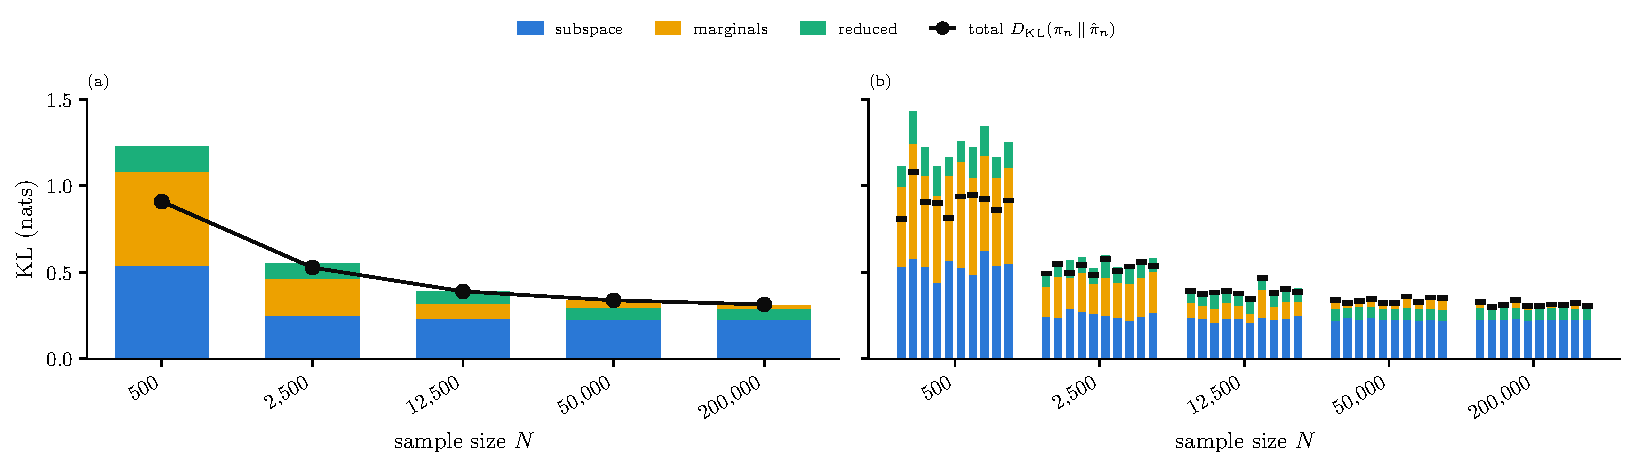
\includegraphics[width=\textwidth]{fig_composite_main_banana.pdf}
\caption{Reference values for the three terms of the decomposition \eqref{eq:kl-three-way} on Example~1 ($d=20$, $r^\star=4$), $10$ draws per $N$; Examples~2 and~3 in Supplement~\ref{S-sm:composite-anatomy}. \emph{(a)}~mean over the $10$ draws. \emph{(b)}~one stacked bar per seed, paired with that seed's reference total (tick mark). The stacked terms omit $R_N$, $\log A$ and the change $\Delta_{\rm cpl}$ of $\mathcal E_{\rm dens}$ between the estimated basis and $\mV_{r,\Lambda}$ (Supplement~\ref{S-sm:composite-anatomy}); for $N \ge 12{,}500$ their sum is on average smaller than the per-draw Monte Carlo error.}
\label{fig:composite-main}
\end{figure*}

The terms behave as \Cref{sec:apriori} predicts. The marginal term decreases with $N$, and the reduced-density and subspace terms level off at limits independent of $N$; the limit of the subspace term depends on $r$ and $\Lambda$ (\Cref{sec:stage1-error}). For $N \ge 12{,}500$ the subspace term is the largest of the three on every example, so at these sample sizes a larger rank or multi-index set reduces the largest term.

\subsection{A priori terms and the a posteriori bound}
\label{sec:exp-aposteriori}

\Cref{fig:stage1-bounds}(a) shows the terms of \eqref{eq:stage1-threeterm} at $N \in \{2500, 50000\}$ for $8$ seeds. The Hermite term is computed from the larger multi-index set $\Lambda_{6,3}$, which lowers it, by \eqref{eq:hier-trunc} (Supplement~\ref{S-sm:experimental-protocol}). On every example the Hermite truncation is the largest term, and only the statistical estimation term decreases with $N$. After squaring and halving, the bound exceeds the reference $\mathcal E_{\rm proj}$ by a factor between $7.5$ and $17.9$ across the examples at $N = 5\times10^4$, and the Hermite term alone is more than half of the bound. \Cref{sec:tightness} measures the part due to the log-Sobolev inequality.

\Cref{fig:stage1-bounds}(b) checks \Cref{cor:aposteriori}. The bound lies above the reference dimension reduction error for every seed and every $N$, in all $96$ estimated models, and the finite-sample term decreases as $N$ grows.

On the same models we evaluate the hierarchical estimate of \Cref{prop:hier-trunc}, enlarging the selected $\Lambda$ once in degree and once in interaction order. The saturation constant $\beta$ depends on the enlargement. When the degree is raised, $\beta$ exceeds $0.98$ on every example, and when the interaction order is raised, $\beta$ lies between $0.62$ and $0.91$. This is consistent with the definition of the examples in Part~I \cite{CAS_partI}, where the dependence has interaction order three or more after the random rotation.

\begin{figure}[t]
\centering
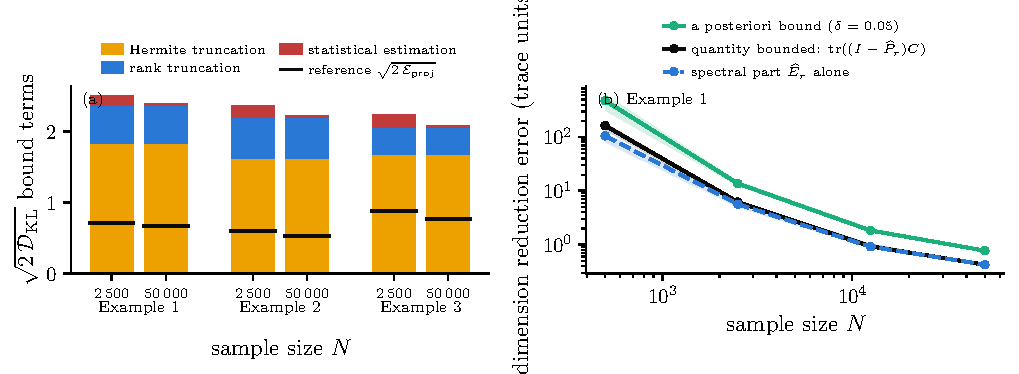
\includegraphics[width=\textwidth]{fig_stage1_bounds.pdf}
\caption{Stage-1 error bounds on Examples~1--3 ($d=20$, $r=4$, $8$ seeds at each $N$). \emph{(a)}~the terms of the a priori bound \eqref{eq:stage1-threeterm} in $\sqrt{2\,\DKL}$ units at $N \in \{2500, 50000\}$; the black line is the reference value $\sqrt{2\,\mathcal E_{\rm proj}}$ in the same units, so the height of the stack above it is the looseness of the bound. \emph{(b)}~the a posteriori bound of \Cref{cor:aposteriori} on Example~1 with $\delta = 0.05$, shown with the bounded quantity $\tr((\mI-\hmP_r)\mC(\whvtheta))$ and with its spectral part $\sum_{i>r}\widehat\lambda_i(\hmC)$ alone; shaded bands span the $8$ seeds. The bound lies above the bounded quantity for every seed and every $N$, and the distance from the spectral part to the bound is the finite-sample term of \eqref{eq:aposteriori}, which decreases as $N$ grows. The Example~2 and~3 values differ from Example~1 by at most $33\%$ for $N \ge 12500$.}
\label{fig:stage1-bounds}
\end{figure}

\subsection{The overall estimate against the reference values}
\label{sec:exp-endtoend}

We compute \eqref{eq:apost-assembled} on the examples and compare each term with the reference value of the corresponding term of \eqref{eq:kl-three-way}. The reduced-density term and its estimate are taken at the basis $\mV_{r,\Lambda}$ of \Cref{sec:exp-reference}, and the bounded subspace term at the estimated basis. Each example is run for $N \in \{500, 2500, 12500, 50000, 200000\}$ with $10$ seeds, $150$ estimated models in all. Each estimate uses $M = 2\times10^5$ held-out residuals and a fixed number of neighbours, $k = 20$ for $r = 4$ and $k = 10$ for $r = 1$ \cite[\S2]{BerrettSamworthYuan2019} (\Cref{sec:limitations}), and reports the standard error of \Cref{cor:apost-den}.

\begin{figure*}[t]
\centering
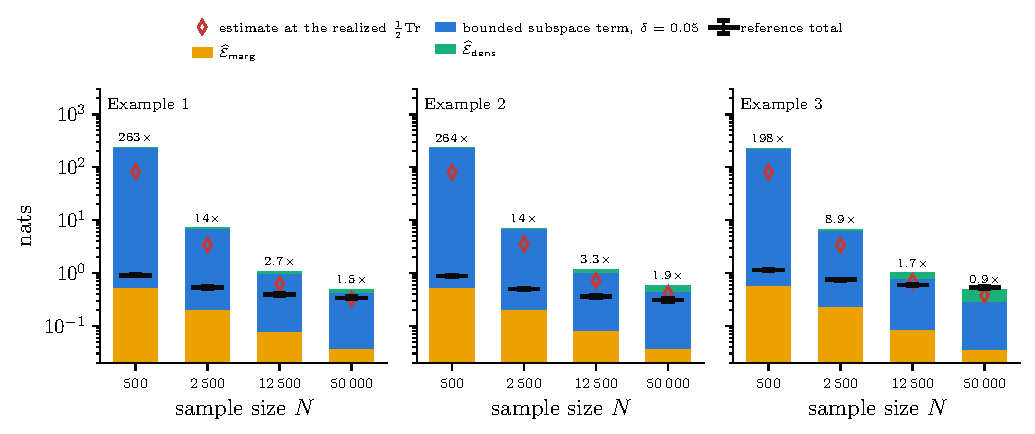
\includegraphics[width=\textwidth]{fig_apost_endtoend.pdf}
\caption{The overall a posteriori estimate \eqref{eq:apost-assembled} against the reference total on Examples~1--3 ($d = 20$, $r = 4$, $\delta = 0.05$; $10$ seeds for the two estimated terms, $8$ for the bounded term). The stacked bar is the estimate, computed from samples alone. The black marker is the reference total $\DKL(\pi_{\vn}\,\|\,\widehat\pi_{\vn})$ with its Monte Carlo standard error. The red diamond is the estimate with the bounded subspace term replaced by the half-trace $\tfrac12\tr((\mI-\hmP_r)\mC(\whvtheta))$, so the distance between diamond and bar is the looseness of the finite-sample bound \eqref{eq:aposteriori}, which comes from Chebyshev's inequality. The number above each bar is the effectivity index, the ratio of the estimate to the reference total. The vertical axis is logarithmic.}
\label{fig:apost-endtoend}
\end{figure*}

In all $150$ estimated models, $\widehat{\mathcal E}_{\rm marg}$ lies within twice the combined standard errors of the reference $\mathcal E_{\rm marg}$. The estimate $\widehat{\mathcal E}_{\rm dens}$ is biased upward by about one combined standard error at every $N$. The bias does not decrease with $N$, which is consistent with the finite-$M$ bias of the entropy estimator \cite[Cor.~4]{BerrettSamworthYuan2019}, since $M$ is the same for every $N$.

In \Cref{fig:apost-endtoend} the effectivity index decreases with $N$ on every example, from the hundreds at $N = 500$ to below $4$ for $N \ge 12{,}500$. At $N = 500$ the bounded term depends, through the fourth moment in \Cref{cor:aposteriori}, on a Stage-1 score estimated from $N_2 = 250$ samples. The estimate exceeds the reference total in $11$ of the $12$ combinations of example and sample size. The exception is Example~3 at the largest $N$, where the index is $0.9$ (\Cref{sec:limitations}).

% =====================================================================
\section{Limitations}
\label{sec:limitations}


\emph{Unverifiable hypotheses.} Condition \textup{(D1)} of \Cref{cor:apost-den} places the unknown reduced density in the smoothness class of \cite{BerrettSamworthYuan2019}. The number of neighbours $k$ is fixed instead of increasing with $M$, so the reported standard error omits part of the variance of the estimator \cite[\S3.4]{BerrettSamworthYuan2019}. Neither condition can be checked from a residual sample; \Cref{sec:exp-endtoend} checks their consequences only on problems with known noise laws.

\emph{The bounded subspace term.} The bound on $\mathcal E_{\rm proj}$ uses Chebyshev's inequality and the Gaussian log-Sobolev inequality, the latter being the main source of looseness (\Cref{sec:tightness}). It bounds $\tr((\mI-\hmP_r)\mC(\whvtheta))$, a trace computed from the parameterized score, and is only as accurate as that score in the complement directions. The exception in \Cref{sec:exp-endtoend}, Example~3 at the largest $N$ with effectivity index $0.9$, comes from this representation; the bound itself exceeds the trace in all $96$ estimated models of \Cref{sec:exp-aposteriori}. On Example~3 the interaction order of the selected multi-index set is too low to represent the score variance in the complement directions. Raising the interaction order by one multiplies $\tr(\mC_\Lambda)$ by $3.7$, whereas raising the degree by one increases it by $0.1\%$, so the estimate depends on the chosen $\Lambda$ as well as on the law.

\emph{Small samples.} At $N = 500$ the bounded term exceeds the reference total by a factor greater than $100$ on every example (\Cref{sec:exp-endtoend}), because the Stage-1 score is estimated from few samples. The errors of the estimated terms are much smaller at every sample size.

\emph{Scope.} The reduction is linear. Dependence that varies along a curved set of directions is represented only through its variation along the chosen subspace, and transport-based reductions \cite{MarzoukMoselhyParnoSpantini2016, ChenArnaudBaptistaZahm2024} are alternatives for such laws. The number of multi-indices $|\Lambda_{K,q}|$ grows as $\binom{d}{q}$ with the interaction order $q$. The analysis assumes a truncation and regularizer fixed in advance; a choice that changes with $N$ is not covered. Every reference value in \Cref{sec:experiments} requires the noise law in closed form, so the behavior of the estimate on residuals from an operational assimilation system is not measured here.

% =====================================================================

\section{Conclusion}
\label{sec:conclusion}

In the problems for which \textsc{Cas} is intended the noise law is unknown, and the error of the estimated density cannot be computed against a reference. We estimate it from the residual sample. The divergence is the exact sum of one term per estimated object (\Cref{prop:exact-decomp}), and the largest term identifies the stage of the estimator that limits the accuracy. The marginal and reduced-density terms are estimated at the parametric rate with computable standard errors (\Cref{cor:apost-den}). The subspace term is bounded by the Stage-1 score covariance (\Cref{cor:aposteriori}), the same matrix that selects the reduction.

On the $150$ estimated models of the examples, whose noise laws are known, the estimated marginal term agrees with its reference value and the reduced-density estimate has a small upward bias. The overall estimate exceeds the reference divergence in $11$ of the $12$ combinations of example and sample size; \Cref{sec:limitations} explains the exception. The conservative step in the a priori bound is the Gaussian log-Sobolev inequality. It overestimates the divergence by a factor between $1.64$ and $1.98$ on the three examples, and on each of them the minimizer of the tighter bound of \cite{LiCuiLiMarzoukZahm2024sharp} lies within $\|\sin\Theta\|_F \le 0.011$ of the top-$r$ eigenbasis of $\mC$ used by \textsc{Cas} (\Cref{sec:tightness}).

For $N \ge 12{,}500$, on all three examples, the largest term of the error is the subspace term. It is then close to a limit set by the rank and the multi-index set and changes little with more samples. Both quantities that set this limit can be computed from the sample. The sum of the trailing eigenvalues is available for every rank from the Stage-1 spectrum, and the Hermite truncation term from the difference between two nested multi-index sets (\Cref{prop:hier-trunc}). The estimate therefore also indicates whether the rank or the multi-index set should be increased.

\section*{Reproducibility}
\label{sec:reproducibility}

Code, saved numerical results, and reproduction instructions are available at \url{https://github.com/joshuawchen/copula_active_subspaces}; the version used for this article is the release tagged \texttt{v1.0-part2}. The script \texttt{reproduce.py} reproduces the figures, using the saved results of the numerical experiments, and recomputes those results on request; the repository README identifies the script behind each figure and table. All settings, including the random states of the reported runs, are recorded in Supplement~\ref{S-sm:experimental-protocol}.


\appendix
\crefalias{section}{appendix}
\crefalias{subsection}{appendix}

% =====================================================================
\section{Proofs of the decomposition and the Stage-1 bounds}
\label{app:thm-trunc}

\begin{proof}[Proof of \Cref{prop:stage1-cert}, \Cref{thm:stage1-rate}, and \eqref{eq:aposteriori-kl}]
Apply the Gaussian-reference bound \eqref{I-eq:kl-trunc} to the basis $\hmV_r^{\mC}$:
\[
  2\,\DKL(\pi_{\vn}\,\|\,\pi_{\vn}(\,\cdot\,;\hmV_r^{\mC}))
  \;\le\;
  \tr\!\bigl((\mI - \hmP_r)\mC\bigr)
  \;=\;
  \|(\mI - \hmP_r)\scS\|_{L^2(\pi_{\vZ})}^2,
\]
the equality using $\mC = \EE_{\pi_{\vZ}}[\scS\scS^\top]$ and idempotence of $\mI-\hmP_r$; halving the left inequality proves \eqref{eq:stage1-cert}. For any score field $\scS'$ with covariance $\mC' := \EE_{\pi_{\vZ}}[\scS'\scS'^\top]$, the triangle inequality in $L^2(\pi_{\vZ};\RR^d)$, non-expansiveness of the orthogonal projector $\mI-\hmP_r$, and $\|(\mI-\hmP_r)\scS'\|_{L^2(\pi_{\vZ})}^2 = \tr((\mI-\hmP_r)\mC')$ bound $\|(\mI-\hmP_r)\scS\|_{L^2}$ by $\|\scS - \scS'\|_{L^2} + \sqrt{\tr((\mI-\hmP_r)\mC')}$, which proves \eqref{eq:finite-sample-kl}; instantiating $\scS' = \widehat\scS$ gives \eqref{eq:aposteriori-kl} of \Cref{cor:aposteriori}. Trace linearity together with Part~I's \Cref{I-cor:optimal-subspace} gives the split \eqref{eq:stage1-split}, that corollary evaluating $\tr((\mI-\mP_r^{\mC})\mC) = \sum_{i>r}\lambda_i(\mC)$ and whose minimality gives $\Delta_{\rm subopt} \ge 0$; the eigengap inequality of Part~I (\Cref{I-prop:diagnostic}), applied to $\mC$ in place of $\mC_\Lambda$, gives uniqueness of the maximizer when $\lambda_r(\mC) > \lambda_{r+1}(\mC)$ and $\Delta_{\rm subopt} = O(\|\sin\Theta(\hmV_r^{\mC},\mV_r^{\mC})\|_F^2)$. Part~I's \Cref{I-prop:diagnostic} identifies $\mP_r^{\Lambda\star}$ as the minimizer of $\tr((\mI-\mP)\mC_\Lambda)$ over rank-$r$ orthogonal projectors, with minimum $\sum_{i>r}\lambda_i(\mC_\Lambda)$, so
\begin{equation}
  \tr\!\bigl((\mI-\hmP_r)\mC_\Lambda\bigr) \;=\; \textstyle\sum_{i>r}\lambda_i(\mC_\Lambda) \;+\; \tr\!\bigl((\mP_r^{\Lambda\star}-\hmP_r)\mC_\Lambda\bigr),
  \label{eq:stage1-decomp}
\end{equation}
with the second summand nonnegative, and $\sqrt{a+b}\le\sqrt a+\sqrt b$ applied to \eqref{eq:finite-sample-kl} at $\scS' = \scS_\Lambda$ and to \eqref{eq:stage1-decomp} gives \eqref{eq:stage1-threeterm}. For \eqref{eq:stage1-estrate}, by Weyl's inequality \cite[Cor.~III.2.6]{Bhatia1997}, the Ky Fan trace extremum \cite[Prob.~III.6.11]{Bhatia1997}, and a rank-$r$ trace bound, $\tr((\mP_r^{\Lambda\star}-\hmP_r)\mC_\Lambda) \le 2r\|\hmC-\mC_\Lambda\|_{\rm op}$, which is $O_p(N^{-1/2}) + O(\tau_N)$ by \eqref{eq:opnorm-rate} of \Cref{lem:score-cov-rate}, a bound that needs no eigengap. The eigengap \textup{(A4)} is needed only for the $\sin\Theta$ rate \eqref{eq:sintheta-rate}, used in the rate-verification experiment of Supplement~\ref{S-sm:rate-real}.
\end{proof}

\begin{proof}[Proof of \eqref{eq:aposteriori} in \Cref{cor:aposteriori}]
Work conditionally on the first half, so the rank transform and $\whvtheta$ are fixed and the second-half scores $\widehat\scS(\vZ^{(n)})$, $n = 1, \dots, N_2$, are i.i.d.\ with $\EE[\widehat\scS\widehat\scS^\top] = \widetilde\mC(\whvtheta)$. The trailing eigenvalues of $\hmC$ satisfy $\sum_{i>r}\widehat\lambda_i(\hmC) = \tr((\mI-\hmP_r)\hmC)$, so
\[
  \tr\!\bigl((\mI-\hmP_r)\widetilde\mC(\whvtheta)\bigr) \;=\; \textstyle\sum_{i>r}\widehat\lambda_i(\hmC) + \tr\!\bigl((\mI-\hmP_r)(\widetilde\mC(\whvtheta) - \hmC)\bigr).
\]
Since $\mI-\hmP_r$ is an orthogonal projector of rank $d-r$, von Neumann's trace inequality \cite{Mirsky1975} bounds the second term by the sum of the $d-r$ largest singular values of $\widetilde\mC(\whvtheta)-\hmC$, and Cauchy--Schwarz bounds that sum by $\sqrt{d-r}\,\|\widetilde\mC(\whvtheta)-\hmC\|_F$; both steps hold for the realized $\hmP_r$. The centered summands $\widehat\scS(\vZ^{(n)})\widehat\scS(\vZ^{(n)})^\top - \widetilde\mC(\whvtheta)$ are i.i.d.\ mean-zero, so
\[
  \EE[\|\hmC - \widetilde\mC(\whvtheta)\|_F^2] \;=\; N_2^{-1}\bigl(\EE[\|\widehat\scS(\vZ)\|_2^4] - \|\widetilde\mC(\whvtheta)\|_F^2\bigr) \;\le\; m_4/N_2,
\]
and Chebyshev's inequality applied to $\|\hmC-\widetilde\mC(\whvtheta)\|_F^2$ gives $\|\hmC-\widetilde\mC(\whvtheta)\|_F \le \sqrt{m_4/(N_2\delta)}$ with probability at least $1-\delta$. Combining these bounds gives \eqref{eq:aposteriori}. The moment $m_4$ is finite for every noise law: $\widehat\scS$ is a fixed polynomial evaluated on the first-half rank transform, whose range is bounded, so $\|\widehat\scS\|_2$ is bounded on the transformed sample space.
\end{proof}

\begin{proof}[Proof of \Cref{prop:hier-trunc}]
$\scS - \scS_{\Lambda'} \perp \scF_{\Lambda'} \ni \scS_{\Lambda'} - \scS_\Lambda$ gives the identity; inserting \textup{(SAT)} into it and rearranging gives \eqref{eq:hier-trunc}. The two estimated fields are fixed quadratics in coefficient vectors that are $O_p(N^{-1/2}) + O(\tau_N)$-consistent by the argument of \Cref{lem:score-cov-rate}, the features have finite fourth moments under \textup{(A2)}, the bilinear form in the two estimation errors has mean zero because the three subsamples are independent, and evaluating the Gram matrix on a subsample not used for estimation removes the in-sample bias. For the sampled score of \eqref{eq:aposteriori-kl}, the triangle inequality applied to \eqref{eq:hier-trunc} together with \Cref{lem:score-cov-rate} gives $\|\scS - \widehat\scS\|_{L^2(\pi_{\vZ})} \le \eta/\sqrt{1-\beta^2} + O_p(N^{-1/2}) + O(\tau_N)$.
\end{proof}

\begin{proof}[Proof of \Cref{prop:exact-decomp} and of the $R_N$ rate of \Cref{prop:apriori-rates}]
By the definitions of \Cref{sec:estimator} and the change of variables along the respective rank transforms, $\pi_{\vn}(\vx) = c^{Z}(\scZ(\vx))\prod_i\pi_i(x_i)$ and $A\,\widehat\pi_{\vn}(\vx) = \widehat c^{Z}(\widehat\scZ(\vx))\prod_i\widehat\pi_i(x_i)$, with $0 < A < \infty$ (Part~I \cite{CAS_partI}). All logarithms below are $\pi_{\vn}$-integrable: $|\log c^{Z}| = |\scL|$ grows polynomially by \textup{(T2)} (Part~I \cite{CAS_partI}) and all polynomial moments are finite under the Gaussian marginals of $\pi_{\vZ}$; $\log\widehat c^{Z}$ is, minus the log-normalizer, the degree-$K_2$ Stage-2 polynomial in $\hmV_r^{\mC\top}\vz$, bounded above by the constraint of the Stage-2 solve (Part~I \cite{CAS_partI}) and of polynomial growth below; and $\EE_{\pi_{\vn}}[|\log(\pi_i/\widehat\pi_i)|] < \infty$ by the integrability of \textup{(M)} (\Cref{sec:estimator}).

\emph{The exact identity.} Pointwise, $\log(\pi_{\vn}/\widehat\pi_{\vn}) = [\log c^{Z}(\scZ) - \log\widehat c^{Z}(\widehat\scZ)] + \sum_i\log(\pi_i/\widehat\pi_i) + \log A$, and $x_i \sim \pi_i$ under $\pi_{\vn}$, so the marginal group contributes $\sum_i\DKL(\pi_i\,\|\,\widehat\pi_i)$ in expectation, and the constant $\log A$ contributes itself. For the copula group, add and subtract $\EE_{\pi_{\vn}}[\log\widehat c^{Z}(\scZ)]$: the transform $\scZ$ pushes $\pi_{\vn}$ forward to $\pi_{\vZ}$, so the first difference equals $\EE_{\pi_{\vZ}}[\log(\pi_{\vZ}/\gauss_d) - \log(\widehat\pi_{\vZ}/\gauss_d)] = \DKL(\pi_{\vZ}\,\|\,\widehat\pi_{\vZ})$, with $\widehat\pi_{\vZ} := \widehat c^{Z}\gauss_d$ normalized by $\widehat Z_r$ (\Cref{sec:apost-density}), and the second difference defines $R_N$. Conditionally on the estimation sample, $\widehat\pi_{\vZ}(\vz) = \widehat c_r^{U}(\vu)\gauss_r(\vu)\,\gauss_{d-r}(\vw)$ is a product in the coordinates $(\vu,\vw) = (\hmV_r^{\mC\top}\vz,\ \hmV_\perp^\top\vz)$, so the chain rule for the KL divergence gives
\[
  \DKL(\pi_{\vZ}\,\|\,\widehat\pi_{\vZ}) \;=\; \DKL(\pi_{\vU}\,\|\,\widehat\pi_{\vU}) + \EE_{\pi_{\vU}}[\DKL(\pi_{\vW\mid\vU}\,\|\,\gauss_{d-r})],
\]
whose second term equals $\DKL(\pi_{\vn}\,\|\,\pi_{\vn}(\,\cdot\,;\hmV_r^{\mC}))$ by the reduced-form identity of Part~I \cite{CAS_partI}, stated there at a fixed subspace and applied here at each realization of $\hmV_r^{\mC}$. Every term above is finite by the integrability recorded at the start of this proof.

\emph{The rate of $R_N$.} By definition $R_N = \EE_{\pi_{\vn}}[\log\widehat c^{Z}(\scZ) - \log\widehat c^{Z}(\widehat\scZ)]$, a difference of one function evaluated at two points, so a Lipschitz bound on $\log\widehat c^{Z}$ and an $L^2$ bound on $\widehat\scZ - \scZ$ suffice. Let $z_N := \Phi^{-1}(N/(N+1))$ be the largest value of the estimated rank transform (Part~I \cite{CAS_partI}), whose empirical CDFs take values in $\{1/(N+1),\dots,N/(N+1)\}$, so $z_N^2 \le 2\log N$ and $\widehat\scZ_i \in [-z_N, z_N]$.

\emph{(a) The transform.} On $\{|\scZ_i| \le z_N\}$, to first order in $\widehat F_i - F_i$, the derivative $1/\gauss_1(\scZ_i)$ of the quantile function and the mean-square bound $\EE[(\widehat F_i - F_i)^2] \le F_i(1-F_i)/N + O(N^{-2})$ give
\[
  \EE\bigl[(\widehat\scZ_i - \scZ_i)^2\bigr]
  \;\le\;
  N^{-1}\!\!\int_{|z|\le z_N}\!\!\frac{\Phi(1-\Phi)}{\gauss_1}\,\mathrm dz \;+\; O(N^{-1})
  \;=\; O(N^{-1}\log N),
\]
the integrand decaying as $1/|z|$. The mean-square bound holds because $N\mathbb F_{i,N}(t)$ is binomial with mean $NF_i(t)$ \cite[\S 19.1]{VanDerVaart1998}, so the empirical distribution function $\mathbb F_{i,N}$ has variance exactly $F_i(1-F_i)/N$, while the rank estimator $\widehat F_i = R_i/(N+1)$ of Part~I \cite{CAS_partI} differs from $\mathbb F_{i,N}$ by at most $1/(N+1)$ pointwise, which contributes the $O(N^{-2})$. The complementary event has probability $2/(N{+}1)$ and conditional second moment $O(\log N)$, contributing $O(N^{-1}\log N)$ as well. Summing over the $d$ coordinates, $\EE[\|\widehat\scZ - \scZ\|_2^2] = O(dN^{-1}\log N)$.

\emph{(b) The estimated log-copula.} On $\{\|\vz\|_\infty \le z_N\}$,
\[
  \begin{aligned}
  \|\nabla\log\widehat c^{Z}(\vz)\|_2
  &\le \|\hvbeta\|_1\max_{\alpha\in\Lambda_r}\ \sup_{\|\vu\|\le\sqrt r\,z_N}\|\nabla H_\alpha(\vu)\| =: L_N,\\
  \EE[L_N^2] &= O\bigl((\log N)^{K_2-1}\bigr),
  \end{aligned}
\]
since $\nabla H_\alpha$ has degree $K_2 - 1$ and $\EE[\|\hvbeta\|_1^2] \le |\Lambda_r|\,\EE[\|\hvbeta\|^2] = O(1)$.

\emph{(c) The complement.} On the event that $|\scZ_i| > z_N$ for some $i$, of probability at most $2d/(N+1)$, the gradient of $\log\widehat c^{Z}$ on the segment from $\widehat\scZ$ to $\scZ$ is bounded by a polynomial in $\|\scZ\|$ with the coefficients of (b), which has all moments, so by Cauchy--Schwarz this event contributes to $\EE[|R_N|]$ at most at the order of the bound below.

Cauchy--Schwarz applied to (a) and (b) gives
\[
  \EE[|R_N|] \;\le\; \bigl(\EE[L_N^2]\bigr)^{1/2}\bigl(\EE[\|\widehat\scZ-\scZ\|_2^2]\bigr)^{1/2}
  \;=\; O\bigl(\sqrt d\,(\log N)^{K_2/2}N^{-1/2}\bigr),
\]
and the same argument per realization gives the $O_p$ rate of \eqref{eq:Delta-marg}. The sum $\sum_i\DKL(\pi_i\,\|\,\widehat\pi_i)$ of the marginal divergences has expectation $O(\sqrt d\,(\log N)^{K_2/2}N^{-1/2})$ by \textup{(M)}, which matches the bound on $R_N$ and gives \eqref{eq:Delta-marg}.

\emph{Expectation and assembly.} Taking the expectation of the identity above over the estimation sample gives $\EE[\DKL(\pi_{\vn}\,\|\,\widehat\pi_{\vn})] = \EE[\mathcal E_{\rm marg}] + \EE[\mathcal E_{\rm proj}] + \EE[\mathcal E_{\rm dens}]$. \Cref{prop:stage1-cert} holds per realization, so $\EE[\mathcal E_{\rm proj}] \le \EE[C_1]$. Conditionally on the half from which $\hmV_r^{\mC}$ is computed, the Stage-2 coefficients are computed from an independent sample projected by a fixed basis, so \eqref{eq:stage2-kl-mean} for that basis gives $\EE[\mathcal E_{\rm dens} \mid \hmV_r^{\mC}] \le \mathcal B_{\rm dens}(\hmV_r^{\mC}) + O(N^{-1})$, with an $O(N^{-1})$ term that does not depend on the basis, since the constants do not. Taking expectations and assembling gives \eqref{eq:composite-kl}.
\end{proof}


\section{The Stage-1 score-covariance rate}
\label{app:sample-proof}

The conditions of \Cref{lem:score-cov-rate} are: \textup{(A1)} $\Lambda$ is finite, excludes the constant mode, and $\pi_{\vZ} > 0$ a.e.; \textup{(A2)} the per-sample score-matching components $\mA(\vZ), \mb(\vZ)$ (Part~I \cite{CAS_partI}) have finite second moments and the Hermite-polynomial features have finite fourth moments under $\pi_{\vZ}$; \textup{(A3)} Stage 1 uses Tikhonov regularization of a fixed strength $\tau_N \ge 0$; \textup{(A4)} the eigengap $\delta_\Lambda := \lambda_r(\mC_\Lambda) - \lambda_{r+1}(\mC_\Lambda)$ is positive. The strength \eqref{I-eq:tikhonov} is data-dependent, $\tau_N \asymp \kappa\|\widehat\mA\|_{\rm op}$ with $\kappa = 10^{-4}$, where $(\widehat\mA, \widehat\mb)$ is the Stage-1 score-matching system, with expectation $(\mA^{d,\star}, \mb^{d,\star})$, and $\|\widehat\mA\|_{\rm op} = \|\mA^{d,\star}\|_{\rm op} + O_p(N^{-1/2})$ under \textup{(A2)}, so the lemma below holds with $\tau_N$ read as the infinite-sample value $\kappa\|\mA^{d,\star}\|_{\rm op}$.

\begin{lemma}[Stage-1 score-covariance rate]
\label{lem:score-cov-rate}
Under Assumption~\ref{I-ass:tempered} of Part~I and the conditions \textup{(A1)}--\textup{(A3)} above, the empirical Stage-1 score covariance $\hmC$ of \eqref{I-eq:Chat-def} satisfies
\begin{equation}
  \|\hmC - \mC_\Lambda\|_{\rm op} \;=\; O_p(N^{-1/2}) \;+\; O(\tau_N)
  \label{eq:opnorm-rate}
\end{equation}
at the Tikhonov regularization strength $\tau_N$ of \textup{(A3)}. If the eigengap condition \textup{(A4)} holds as well, then the estimated Stage-1 basis satisfies
\begin{equation}
  \|\sin\Theta(\hmV_r^{\mC}, \mV_{r,\Lambda})\|_F \;=\; O_p(N^{-1/2}) \;+\; O(\tau_N/\delta_\Lambda).
  \label{eq:sintheta-rate}
\end{equation}
\end{lemma}

\begin{proof}[Proof of \Cref{lem:score-cov-rate}]
Under Assumption~\ref{I-ass:tempered} with a finite $\Lambda$, every entry of $\mA(\vz), \mb(\vz)$, and the Hermite-polynomial features is polynomial in $\vz$ of bounded degree, so the Gaussian marginals of $\vZ$ give the moment conditions (A2). The entries of $\widehat\mA$, $\widehat\mb$ and $\hmC$ are averages over the rank-transformed sample, whose points depend on one another through the ranks. Averages of polynomials in the normal scores of the ranks are asymptotically normal at rate $N^{-1/2}$ \cite{GenestGhoudiRivest1995}, with an asymptotic covariance that includes the effect of the ranks, so the central limit theorem used below applies to them with that covariance. Positive definiteness of $\mA^{d,\star}$ under (A1) follows from $\mathbf a^\top\mA^{d,\star}\mathbf a = \EE_{\pi_{\vZ}}[\|\sum_\alpha a_\alpha\nabla H_\alpha(\vZ)\|^2]$ together with constant-mode exclusion.

Let $\bm\theta_{\tau_N} := (\mA^{d,\star} + \tau_N\mI)^{-1}\mb^{d,\star}$ be the infinite-sample regularized coefficient and $\bm\theta^{d,\star}_\Lambda := (\mA^{d,\star})^{-1}\mb^{d,\star}$ the unregularized truth. The regularized normal equation $(\widehat\mA + \tau_N\mI)\widehat\theta_N = \widehat\mb$ is a regularized M-estimator with infinite-sample solution $\bm\theta_{\tau_N}$; differentiability of $(\mA,\mb)\mapsto(\mA+\tau_N\mI)^{-1}\mb$ at $(\mA^{d,\star},\mb^{d,\star})$, which is the hypothesis of \cite[Thm.~3.1]{VanDerVaart1998}, together with the multivariate CLT and the delta method gives $\widehat\theta_N - \bm\theta_{\tau_N} = O_p(N^{-1/2})$, the strength $\tau_N$ being fixed by \textup{(A3)} so that neither the map nor its centering varies with $N$, and at fixed strength $\bm\theta_{\tau_N} - \bm\theta^{d,\star}_\Lambda = -\tau_N(\mA^{d,\star} + \tau_N\mI)^{-1}\bm\theta^{d,\star}_\Lambda = O(\tau_N)$; the weight $\mR_{H^2} = \tau_N\diag(|\alpha|_1^2)$ of \eqref{I-eq:tikhonov} replaces $\tau_N\mI$ by $\tau_N\mD$ with $\|\mD\|_{\rm op} \le K_1^2$, and both parts hold verbatim with $\tau_N$ carrying that factor. The identity $aa^\top - bb^\top = (a-b)a^\top + b(a-b)^\top$ at $a = \mPsi\widehat\theta_N$, $b = \mPsi\bm\theta^{d,\star}_{\Lambda}$, for the gradient matrix $\mPsi$ with columns $\nabla H_\alpha$ and bounded fourth moments of its columns, gives $\|\hmC - \mC_\Lambda\|_{\rm op} = O_p(N^{-1/2}) + O(\tau_N)$; for $\tau_N < \delta_\Lambda$ the eigengap of the perturbed matrix is positive, and the Davis--Kahan theorem \cite[Thm.~2]{YuWangSamworth2015} applied with the operator-norm bound gives \eqref{eq:sintheta-rate}.
\end{proof}

% =====================================================================
\section{Proof of the a posteriori divergence estimate}
\label{app:apost-den}

\begin{proof}[Proof of \Cref{cor:apost-den}]
By \cite[\S4, following Thm.~8]{BerrettSamworthYuan2019}, under \textup{(D1)} the weighted estimator is asymptotically linear with efficient influence function $-\log\pi_{\vU} - H(\pi_{\vU})$:
$\widehat H^{w}_M - H(\pi_{\vU}) = M^{-1}\sum_m\bigl[-\log\pi_{\vU}(\vu_m) - H(\pi_{\vU})\bigr] + o_p(M^{-1/2})$.
The cross-entropy term of \eqref{eq:apost-est} is exactly an i.i.d.\ sample mean under \textup{(D3)}, so subtracting,
\[
  \widehat{\mathcal E}_{\rm dens} - \mathcal E_{\rm dens}
  \;=\;
  \frac1M\sum_{m=1}^M\Bigl[\log\frac{\pi_{\vU}(\vu_m)}{\widehat\pi_{\vU}(\vu_m)} - \mathcal E_{\rm dens}\Bigr] \;+\; o_p(M^{-1/2}),
\]
an average of i.i.d.\ mean-zero terms with variance $\sigma_{\rm den}^2 < \infty$ by \textup{(D2)}. The central limit theorem and Slutsky's lemma give \eqref{eq:apost-clt}; \cite[Thm.~1]{BerrettSamworthYuan2019} together with the law of large numbers on the cross-entropy gives consistency. Minkowski's inequality applied to $\log\pi_{\vU} - \log\widehat\pi_{\vU}$ in $L^2(\pi_{\vU})$ gives the variance bound, with the first term estimated by the variance estimator of \cite[\S2]{BerrettSamworthYuan2019}. For $r = 1$ the weight class has no $\Gamma$-constraints, and the unweighted estimator arises at $w = e_k$.
\end{proof}

% =====================================================================
\section{Stage-2 regularizer: proofs and constant selection}
\label{app:bisc-ridge}

The estimator is the finite-basis instance of Tikhonov-regularized score matching \cite[Thms.~4 and~5]{Sriperumbudur2017}, which attains parametric rates in finite dimension \cite[Thm.~7(iii)]{Sriperumbudur2017}. The per-mode design follows the eigenbasis bias--variance analysis of ridge estimators \cite{HoerlKennard1970}, cf.\ \cite[\S3.4]{HastieTibshiraniFriedman2009}, and the degree-weighted penalty is Tikhonov regularization in a Hermite--Sobolev Hilbert scale \cite{EnglHankeNeubauer1996}. New here are the bound on the noise in each degree class (\Cref{cor:per-class-cov-bound}), which holds exactly for the Hermite score-matching integrands and can be evaluated from the sample, and the two-regime form of \Cref{thm:ccsm-rate}. Throughout, $\Lambda^{(k)} := \{\alpha \in \Lambda_r : |\alpha|_1 = k\}$ denotes the degree-$k$ class, of cardinality $p_k := |\Lambda^{(k)}|$; $\widehat\mM := \widehat\mA_r + \mR(\widehat\mA_r)$ denotes the regularized Gram matrix, with $\mR(\widehat\mA_r) = \mR_{\rm samp}(\widehat\mA_r) + \mR_{\rm curv}(\widehat\mA_r)$ as in \eqref{I-eq:R-combined}; and $\widehat\mB \in \RR^{r \times |\Lambda_r|}$ denotes the empirical centering matrix of \Cref{sec:ridge}.

\paragraph{Standing hypotheses} The proofs in this appendix use the following structural conditions on the Stage-2 problem.
\begin{itemize}
\item[\textbf{(H1)}] \emph{Bounded reduced factor on $\RR^r$.} The reduced factor $c_r^{U} := \pi_{\vU}/\gauss_r$ is essentially bounded, $C_\star := \mathrm{ess\,sup}\,c_r^{U} < \infty$. This condition is stronger than (T1), and the example problems of \Cref{sec:exp-benchmark} satisfy it; it implies the finite second moments of $b_\alpha(\vU), A_{\alpha\beta}(\vU)$ from the Hermite score-matching system (Part~I \cite{CAS_partI}) under $\pi_{\vU}$.
\item[\textbf{(H2)}] \emph{Sobolev regularity of the exact reduced log-copula.} The function $\scL_r = \log c_r^{U}$ lies in $H^s_{\gauss}(\RR^r)$ for some $s > 1/2$: writing $\vartheta_\alpha := \langle\scL_r, H_\alpha\rangle_{L^2(\gauss_r)}$ for its Hermite coefficients over all $\alpha \in \NN_0^r$, $\|\scL_r\|_{H^s_{\gauss}}^2 = \sum_\alpha |\alpha|_1^{2s}\vartheta_\alpha^2 =: M^2 < \infty$. The Sobolev bound \eqref{eq:Hs-norm} on per-mode signal magnitudes follows from this.
\end{itemize}

\smallskip
\noindent The analysis fixes the basis $\mV_r$ and uses the exact rank transform, so that the projected sample is drawn independently from $\pi_{\vU}$, as in \Cref{I-prop:centering} of Part~I. \Cref{prop:apriori-rates} applies it conditionally on a basis computed from an independent half of the sample. With the estimated rank transform, the entries of $\widehat\mA_r$, $\widehat\mb_r$ and $\widehat\mB$ are averages of polynomials in the normal scores of the ranks, asymptotically normal at the same rate \cite{GenestGhoudiRivest1995}, so the rates below carry over at leading order, but the constants, which use the variances of the score-matching integrands under $\pi_{\vU}$ (\Cref{cor:per-class-cov-bound}), are those of the exact transform.

\subsection{The Stage-2 regularizer}
\label{sec:ridge}

Part~I constructs the Stage-2 regularizer $\mR$ and selects its constants by validation score-matching risk (\Cref{I-sec:ridge}). The regularizer is diagonal and computed from the data. Its two terms control two sources of error in the unregularized normal equations $\widehat\mA_r\hvbeta = \widehat\mb_r$, the sampling noise in the smallest eigenvalues of $\widehat\mA_r$ and the truncation residual propagated through $\widehat\mA_r^{-1}$.

\paragraph{Form}
Part~I's regularizer is $\mR(\widehat\mA_r) = \mR_{\rm samp}(\widehat\mA_r) + \mR_{\rm curv}(\widehat\mA_r)$ of \eqref{I-eq:R-combined}, constant on each degree class $\Lambda^{(k)}$ with entry $\nu^{(k)} := C_{\rm samp}\widehat\sigma_k^2 + C_{\rm curv}\|\widehat\mA_r\|_{\rm op}k^2$, where $\widehat\sigma_k^2 := \tfrac{1}{N}\tr(\widehat\mA_r^{(k,k)})$ is the degree-class variance scale. The two terms are of different orders in $N$: $\widehat\sigma_k^2 \asymp k\,p_k/N$ decreases to $0$ with $N$, whereas $\|\widehat\mA_r\|_{\rm op}$ has an $N$-independent limit, and the two regimes of \Cref{thm:ccsm-rate} follow from that difference. The exponent $2$ in the $|\alpha|_1^2$ weighting is fixed, and neither the theory nor the constant selection adapts it to the unknown $s$ of \textup{(H2)}.

The two terms are derived from the regularizer $\nu_i^\star$ that is optimal for each mode of the estimation term (\Cref{app:bias-var}), which depends on the unknown $\widetilde\Sigma$ and on the unknown signal magnitudes $(\theta^{r,\star}_i)^2$; the regularizer does not affect the truncation term. $\mR_{\rm samp}$ replaces the variance in the numerator of $\nu_i^\star$ by a bound for each degree class computed from the sample, $\widetilde\Sigma_{ii} \le C_{\rm samp}^{(k)}\,\widehat\sigma_k^2$ with $C_{\rm samp}^{(k)} \le C_{\rm samp}\,k/p_k$ (\Cref{cor:per-class-cov-bound}), and $\mR_{\rm curv}$ replaces the signal magnitudes by the decay $\vartheta_\alpha^2 \le M^2|\alpha|_1^{-2s}$, $M^2 := \|\scL_r\|^2_{H^s_{\gauss}}$, of \textup{(H2)}, with $\lambda_i \asymp |\alpha|_1$ per degree class.

Alongside the regularizer, Part~I imposes the centering constraint $\widehat\mB\hvbeta = 0$ through the empirical centering matrix $\widehat\mB$, $\widehat B_{j\alpha} := \tfrac{1}{N}\sum_n \partial_j H_\alpha(\vu^{(n)})$; \Cref{I-prop:centering} gives its finite-sample effect.

\paragraph{Stage-2 estimator}
The estimator is the constrained minimizer of Part~I (\Cref{I-sec:ridge}); with the centering constraint alone, its solution is given in closed form by \eqref{I-eq:stage2-closedform} in terms of the regularized Gram matrix $\widehat\mM$. The remaining constraints of Part~I bound the estimated potential (\Cref{I-sec:ridge-solve}), the full constraint set is convex, and the estimator equals \eqref{I-eq:stage2-closedform} whenever the centering-only solution satisfies the bound. \Cref{lem:constraints} relates the two solutions in general.

\emph{The constants.} The theoretical scales are $C_{\rm samp}^{(k)} \le C_\Sigma\,k/p_k$ (\Cref{cor:per-class-cov-bound}) and $C_{\rm curv} \asymp (NM^2\|\mA^\star\|_{\rm op})^{-1}$, from \eqref{eq:Hs-norm} substituted into \eqref{eq:rho-optimal}, and the prefactors involve the unknown $C_\Sigma$ of \eqref{eq:CSigma-def} and $M^2$. Part~I selects the two constants for each estimate by minimizing the validation score-matching objective (\Cref{I-sec:ridge}), whose expectation equals, up to an additive constant free of $\vbeta$, the Fisher divergence bounded in \Cref{thm:ccsm-rate} (\Cref{I-lem:hyv-sm}). \Cref{thm:ccsm-rate} holds for each fixed pair. The selected pair $\widehat{\mathbf c}$ depends on the sample but lies in the set $\mathcal P$ of the $5\times5$ grid of Part~I \cite{CAS_partI}, and, with $\hvbeta_{\mathbf c}$ the estimate for the pair $\mathbf c$, $\mathcal J_{\rm est}(\hvbeta_{\widehat{\mathbf c}}) \le \sum_{\mathbf c\in\mathcal P}\mathcal J_{\rm est}(\hvbeta_{\mathbf c})$ for every realization. The expected error at the selected pair is therefore at most $|\mathcal P|$ times the largest bound of \Cref{thm:ccsm-rate} over $\mathcal P$, whatever the selection rule. We do not claim that the selection is optimal.

\subsection{Truncation and estimation error}
\label{app:bias-var}

Throughout this appendix the Fisher divergence $\mathcal J(\widehat\scL_r) := \|\nabla(\widehat\scL_r - \scL_r)\|^2_{L^2(\pi_{\vU})}$ satisfies $\mathcal J(\widehat\scL_r) = 2J(\hvbeta)$, where $J$ is the halved Fisher divergence of Part~I, eq.~\eqref{I-eq:JW-pop}. The factor of $2$ is included in the constants of \Cref{thm:ccsm-rate}.

The Fisher divergence of the estimated $\widehat\scL_r = \sum_{\alpha\in\Lambda_r}\widehat\theta^r_\alpha H_\alpha$ splits, by the triangle inequality in $L^2(\pi_{\vU};\RR^r)$, into a truncation term and an estimation term:
\begin{equation}
  \sqrt{\mathcal J(\widehat\scL_r)} \;\le\; \underbrace{\bigl\|\nabla(\scL_r - \scL_r^\star)\bigr\|_{L^2(\pi_{\vU})}}_{\sqrt{\mathcal J_{\rm trunc}}} \;+\; \underbrace{\bigl\|\nabla(\scL_r^\star - \widehat\scL_r)\bigr\|_{L^2(\pi_{\vU})}}_{\sqrt{\mathcal J_{\rm est}(\hvbeta)}},
  \label{eq:triangle}
\end{equation}
where $\scL_r^\star := \sum_{\alpha\in\Lambda_r}\theta^{r,\star}_\alpha H_\alpha$ is the infinite-sample Stage-2 minimizer over $\Lambda_r$, whose gradient is the $L^2(\pi_{\vU})$-projection of $\nabla\scL_r$ onto $\mathrm{span}\{\nabla H_\alpha : \alpha\in\Lambda_r\}$; its coefficients $\theta^{r,\star}_\alpha$ coincide with the Hermite coefficients $\vartheta_\alpha$ of \textup{(H2)} exactly when $\pi_{\vU} = \gauss_r$. The truncation term satisfies, under \textup{(H1)}--\textup{(H2)} with $s>1/2$, $\mathcal J_{\rm trunc} \le C_\star\,K^{-(2s-1)}\|\scL_r\|^2_{H^s_{\gauss}}$ with $K := \min\{|\alpha|_1 : \alpha\notin\Lambda_r,\ \vartheta_\alpha \ne 0\}$: projection optimality bounds $\mathcal J_{\rm trunc}$ by the candidate $\sum_{\alpha\in\Lambda_r}\vartheta_\alpha H_\alpha$, the bound $\pi_{\vU} \le C_\star\gauss_r$ of \textup{(H1)} transfers the residual to $L^2(\gauss_r)$, and $\gauss_r$-orthogonality evaluates it as $\sum_{\alpha\notin\Lambda_r}|\alpha|_1\vartheta_\alpha^2 \le K^{-(2s-1)}M^2$, using $|\alpha|_1 \geq K$ for every mode with a nonzero coefficient. On $\Lambda_{K_2,q_2}$, $K = K_2 + 1$ exactly when the omitted modes (the linear $e_j$ and the interactions with $|\alpha|_0 > q_2$) have zero coefficients. Any nonzero coefficient of an omitted mode lowers $K$ to the total degree of that mode, so $K = 1$ if some $\vartheta_{e_j} \ne 0$, which zero-mean marginals of $\pi_{\vU}$ do not exclude.

For the estimation term, write $\widehat\mA_r = \mA^\star + \bm\Xi_A$ and $\widehat\mb_r = \mb^\star + \bm\xi_b$ with $\EE[\bm\Xi_A] = 0$, $\EE[\bm\xi_b] = 0$, $\mb^\star = \mA^\star\bm\theta^{r,\star}$, and consider $\hvbeta(\mR) := (\widehat\mA_r + \mR)^{-1}\widehat\mb_r$, whose estimation error $\hvbeta(\mR) - \bm\theta^{r,\star} = (\widehat\mA_r + \mR)^{-1}\bigl[\bm\xi_b - \bm\Xi_A\bm\theta^{r,\star} - \mR\bm\theta^{r,\star}\bigr]$. In the bracket, $\bm\xi_b$ and $\bm\Xi_A\bm\theta^{r,\star}$ are sampling noise and $\mR\bm\theta^{r,\star}$ is the regularization bias. Diagonalizing $\mA^\star$ with eigenvalues $\lambda_i$ and components $\theta^{r,\star}_i$, restricting $\mR$ to be diagonal in this eigenbasis with entries $\nu_i$, the leading-order expected estimation error in the $\mA^\star$-norm (dropping the $O(N^{-1})$ Neumann remainder of \Cref{lem:unc-bias}) is
\begin{equation}
  \EE[\mathcal J_{\rm est}(\hvbeta(\mR))] \;=\; \sum_i \frac{\lambda_i\bigl[\nu_i^2(\theta^{r,\star}_i)^2 + \widetilde\Sigma_{ii}\bigr]}{(\lambda_i + \nu_i)^2} \;+\; O(N^{-1}),
  \label{eq:bias-var-fisher}
\end{equation}
where $\widetilde\Sigma := \Cov(\bm\xi_b - \bm\Xi_A\bm\theta^{r,\star})$ is the score-equation residual covariance in the $\mA^\star$ eigenbasis. Expression \eqref{eq:bias-var-fisher} is the eigenbasis bias-variance decomposition of the ridge estimator \cite{HoerlKennard1970}, cf.\ \cite[\S3.4]{HastieTibshiraniFriedman2009}. Minimizing the leading-order expression mode by mode gives the optimal regularizer, which cannot be computed because it depends on unknown quantities,
\begin{equation}
  \nu_i^\star \;=\; \frac{\widetilde\Sigma_{ii}}{\lambda_i\,(\theta^{r,\star}_i)^2},
  \label{eq:rho-optimal}
\end{equation}
and the regularizer of \Cref{sec:ridge} is built from bounds on the two unknown quantities in it. The Sobolev assumption further yields the per-mode signal bound
\begin{equation}
  \vartheta_\alpha^2 \;\le\; M^2\,|\alpha|_1^{-2s},
  \qquad M^2 := \|\scL_r\|^2_{H^s_{\gauss}} \;=\; \sum_\alpha |\alpha|_1^{2s}\vartheta_\alpha^2.
  \label{eq:Hs-norm}
\end{equation}
The regularizer design of \Cref{sec:ridge} applies the same decay to the minimizer components $\theta^{r,\star}_i$ in \eqref{eq:rho-optimal}, which is exact when $\pi_{\vU} = \gauss_r$ and is used as an approximation otherwise, and the selected constants $(C_{\rm samp}, C_{\rm curv})$ compensate for the difference.

\begin{lemma}[Bias of the unconstrained regularized estimator]
\label{lem:unc-bias}
Under (H1), the Neumann expansion of $\hvbeta_{\rm unc}(\mR) := \widehat\mM^{-1}\widehat\mb_r$ with $\widehat\mM = (\mA^\star+\mR) + \bm\Xi_A$, $\widehat\mb_r = \mb^\star + \bm\xi_b$, and $\mb^\star = \mA^\star\bm\theta^{r,\star}$ (the stochastic counterpart of the deterministic ridge-bias formula, cf.\ \cite[\S 3.4]{HastieTibshiraniFriedman2009}) gives
\begin{equation}
  \hvbeta_{\rm unc}(\mR) - \bm\theta^{r,\star}
  \;=\;
  -\,(\mA^\star+\mR)^{-1}\mR\,\bm\theta^{r,\star}
  \;+\;
  (\mA^\star+\mR)^{-1}\bigl[\bm\xi_b - \bm\Xi_A\,\bm\theta^{r,\star}\bigr]
  \;+\;
  \mathfrak R_N,
  \label{eq:unc-expansion}
\end{equation}
with $\mathfrak R_N = -(\mA^\star+\mR)^{-1}\bm\Xi_A\,(\hvbeta_{\rm unc} - \bm\theta^{r,\star})$ exactly, so that pathwise $\|\mathfrak R_N\| = O_p\bigl(N^{-1/2}\|(\mA^\star+\mR)^{-1}\mR\bm\theta^{r,\star}\| + N^{-1}\bigr)$ and, assuming $\EE[\|\hvbeta_{\rm unc}\|^2] = O(1)$, $\|\EE[\mathfrak R_N]\| = O(N^{-1})$, since the part of $\mathfrak R_N$ that is first order in the noise has mean zero. In particular, $\EE[\hvbeta_{\rm unc}(\mR)] - \bm\theta^{r,\star} = -(\mA^\star+\mR)^{-1}\mR\,\bm\theta^{r,\star} + O(N^{-1})$.
\end{lemma}

\begin{proof}
With $M := \mA^\star + \mR$, the resolvent identity $\widehat\mM^{-1} = M^{-1} - M^{-1}\bm\Xi_A\widehat\mM^{-1}$ and $M^{-1}\mb^\star = M^{-1}(M - \mR)\bm\theta^{r,\star} = \bm\theta^{r,\star} - M^{-1}\mR\bm\theta^{r,\star}$ give \eqref{eq:unc-expansion} with the exact remainder $\mathfrak R_N = -M^{-1}\bm\Xi_A(\hvbeta_{\rm unc} - \bm\theta^{r,\star})$. The pathwise order follows by inverting the fixed-point form $(\mI + M^{-1}\bm\Xi_A)(\hvbeta_{\rm unc} - \bm\theta^{r,\star}) = -M^{-1}\mR\bm\theta^{r,\star} + M^{-1}[\bm\xi_b - \bm\Xi_A\bm\theta^{r,\star}]$ on the event $\|M^{-1}\bm\Xi_A\|_{\rm op} \le 1/2$, of probability $1-o(1)$ by Markov. For the expectation, one substitution of the fixed-point form expresses $\mathfrak R_N$ as a mean-zero term plus two terms whose expectations are $O(N^{-1})$: covariances of mean-zero sample averages, finite under the polynomial moments of \textup{(H1)}, and a term bounded by Cauchy--Schwarz with $\|M^{-1}\|_{\rm op} \le 1/\lambda_{\min}(\mA^\star)$, $\EE[\|\bm\Xi_A\|_{\rm op}^4] = O(N^{-2})$, and the assumed second moment.
\end{proof}

\subsection{Per-class noise bound for the variance regularizer}
\label{app:cv-bound}

\paragraph{Setup} Let $\bm\xi(\vu) := \mathbf b(\vu) - \mathbf A(\vu)\bm\theta^{r,\star}$ be the per-sample score-matching residual on $\RR^r$, with $\mathbf A, \mathbf b$ the Hermite score-matching integrands (Part~I \cite{CAS_partI}). The empirical residual is $\bm\xi_b - \bm\Xi_A\bm\theta^{r,\star} = N^{-1}\sum_n\bm\xi(\vU^{(n)})$, with covariance $\bm\Sigma := N^{-1}\Cov_{\pi_{\vU}}\bm\xi(\vU)$. Denote by $\widetilde{\bm\Sigma}$ the same covariance expressed in the $\mA^\star$-eigenbasis; its diagonal entries $\widetilde\Sigma_{ii}$ appear in the optimal regularizer of the infinite-sample formulation \eqref{eq:bias-var-fisher}.

\paragraph{From the exact class trace to a sample statistic} The infinite-sample class trace equals $\tr(\mA^{\star,(k,k)}) = \sum_{\alpha\in\Lambda^{(k)}}\sum_{j=1}^r\alpha_j\,\EE_{\pi_{\vU}}[H_{\alpha-e_j}^2(\vU)]$ for each $k$, bounded above under (H1) by $C_\star \sum_{\alpha\in\Lambda^{(k)}}\sum_j\alpha_j = C_\star\,k\,p_k$ (write $C_+ := C_\star$ for this upper class-trace constant), and bounded below by a positive constant times $k\,p_k$ provided the class is non-degenerate ($\EE_{\pi_{\vU}}[H_{\alpha-e_j}^2] \ge C_- > 0$ on $\Lambda^{(k)}$, which holds when $\pi_{\vU}$ has full support and $\Lambda^{(k)}$ is $L^2(\pi_{\vU})$-independent). Hence
\begin{equation}
  \tr(\mA^{\star,(k,k)}) \;\asymp\; k\,p_k.
  \label{eq:class-trace-asymp}
\end{equation}
The empirical statistic $\widehat\sigma_k^2 := N^{-1}\tr(\widehat\mA_r^{(k,k)})$ converges to $\EE[\widehat\sigma_k^2] = N^{-1}\tr(\mA^{\star,(k,k)})$ at rate $O_p(N^{-1/2})$ under the second-moment assumption in (H1).

\begin{corollary}[Per-mode variance bound computable from the sample]
\label{cor:per-class-cov-bound}
Under (H1) and the class-trace asymptotics \eqref{eq:class-trace-asymp}, set $C_b := 2$ and $C_A := 2K_b^2 K_{\max}$, with $K_b$ the Hermite hypercontractivity constant \cite{Janson1997gaussian} for total degree $\le K_{\max} := \max_{\beta\in\Lambda_r}|\beta|_1$ (finite for any fixed multi-index set). Then the constant
\begin{equation}
  C_\Sigma \;:=\; \frac{C_\star\,(C_b + C_A\|\bm\theta^{r,\star}\|^2)}{C_-},
  \label{eq:CSigma-def}
\end{equation}
depending only on $(C_\star, K_{\max}, K_b, \|\bm\theta^{r,\star}\|, C_-)$, satisfies, for every $\alpha\in\Lambda^{(k)}$,
\begin{equation}
  \bm\Sigma_{\alpha\alpha}
  \;\le\;
  C_\Sigma\,\widehat\sigma_k^2 \cdot \frac{k}{p_k}
  \;+\;
  O_p(N^{-3/2}).
  \label{eq:per-class-bound}
\end{equation}
The proof of \Cref{thm:ccsm-rate} uses the bound in the canonical Hermite basis. The discussion of \eqref{eq:rho-optimal} also uses it as an approximation to the entries $\widetilde\Sigma_{ii}$ in the $\mA^\star$-eigenbasis. This approximation is not used in any proof.
\end{corollary}

\begin{proof}
\emph{(i)} The Hermite three-term recurrence $u_j H_{\alpha-e_j} = \sqrt{\alpha_j}H_\alpha + \sqrt{\alpha_j-1}H_{\alpha-2e_j}$ collapses the $j$-th summand of $b_\alpha$ (Part~I \cite{CAS_partI}) to $\alpha_j H_\alpha$, so $b_\alpha = |\alpha|_1 H_\alpha = k H_\alpha$ and $\Var_{\pi_{\vU}}[b_\alpha] \le \EE_{\pi_{\vU}}[b_\alpha^2] = k^2\EE_{\pi_{\vU}}[H_\alpha^2] \le C_\star k^2$ by (H1) and Hermite $L^2(\gauss_r)$-orthonormality. \emph{(ii)} With $(\mathbf A\bm\theta^{r,\star})_\alpha = \nabla H_\alpha\cdot\nabla\scL_r^\star$, pointwise Cauchy--Schwarz, the $L^4$--$L^2$ Hölder split, and Hermite hypercontractivity $\|f\|^2_{L^4(\gauss_r)} \le K_b\|f\|^2_{L^2(\gauss_r)}$ at fixed degree, with $\|\nabla H_\alpha\|^2_{L^2(\gauss_r)} = k$ and $\|\nabla\scL_r^\star\|^2_{L^2(\gauss_r)} \le K_{\max}\|\bm\theta^{r,\star}\|^2$, give $\Var_{\pi_{\vU}}[(\mathbf A\bm\theta^{r,\star})_\alpha] \le C_\star K_b^2 k^2 K_{\max}\|\bm\theta^{r,\star}\|^2$. \emph{(iii)} $\Var[\xi_\alpha] \le 2\Var[b_\alpha] + 2\Var[(\mathbf A\bm\theta^{r,\star})_\alpha]$ gives $\bm\Sigma_{\alpha\alpha} = N^{-1}\Var_{\pi_{\vU}}[\xi_\alpha] \le N^{-1}C_\star k^2(C_b + C_A\|\bm\theta^{r,\star}\|^2)$. Combining with the lower bound $\EE[\widehat\sigma_k^2] \ge C_-\,p_k\,k/N$ from \eqref{eq:class-trace-asymp}, giving $k^2/N \le k\,\widehat\sigma_k^2/(C_-\,p_k) + O_p(N^{-3/2})$, yields \eqref{eq:per-class-bound} with $C_\Sigma$ as defined.
\end{proof}

\subsection{Error bound for the Stage-2 estimator}
\label{app:excess-fisher}

\begin{theorem}[Stage-2 Fisher divergence error bound and regularizer scaling]
\label{thm:ccsm-rate}
Under (H1)--(H2), let $\hvbeta$ be the solution \eqref{I-eq:stage2-closedform} of the Stage-2 problem with the centering constraint alone, with regularizer \eqref{I-eq:R-combined} for any constants $(C_{\rm samp}, C_{\rm curv}) > 0$. The bound holds to leading order. The terms $\mathcal V$ and $\mathcal B$ below, whose sum is the estimation term $\mathcal E_{\rm est}$ of \Cref{thm:stage2-kl}, determine the scaling of the regularizer used in \Cref{sec:ridge}, and the remaining contributions are collected in the $O(N^{-1})$ remainder. Define the sample size at which the two expressions in \eqref{eq:V-piecewise} below are equal,
\begin{equation}
  N_{\rm cross}
  \;:=\;
  \frac{C_V^{\rm curv}\,C_{\rm samp}\,|\Lambda_r|}{C_V^{\rm samp}\,C_{\rm curv}},
  \label{eq:Ncross}
\end{equation}
with the constants $C_V^{\rm samp}$ and $C_V^{\rm curv}$ given in the proof.
Then
\begin{equation}
  \EE[\mathcal J(\hvbeta)] - \mathcal J(\bm\theta^{r,\star})
  \;\le\;
  \mathcal V(C_{\rm samp}, C_{\rm curv}, N)
  \;+\;
  \mathcal B(C_{\rm curv})
  \;+\;
  C_{\rm ctr}\,\mathcal J_{\rm trunc}
  \;+\; O(N^{-1}),
  \label{eq:ccsm-rate}
\end{equation}
with the variance term equal to the smaller of two bounds, each valid for every $N$,
\begin{equation}
  \mathcal V(C_{\rm samp}, C_{\rm curv}, N)
  \;=\;
  \begin{cases}
    \dfrac{C_V^{\rm samp}}{C_{\rm samp}}, & N \le N_{\rm cross}, \\[4pt]
    \dfrac{C_V^{\rm curv}\,|\Lambda_r|}{N\,C_{\rm curv}}, & N > N_{\rm cross},
  \end{cases}
  \label{eq:V-piecewise}
\end{equation}
$N$-independent bias term
\begin{equation}
  \mathcal B(C_{\rm curv})
  \;=\;
  C_B\,C_{\rm curv}^2\,\|\mA^\star\|_{\rm op}^2\,K_{\max}^4\,\|\bm\theta^{r,\star}\|^2.
  \label{eq:B-bound}
\end{equation}
The constants $C_V^{\rm samp}, C_V^{\rm curv}, C_B$ depend on $\lambda_{\min}(\mA^\star)$, $K_{\max}$, $C_+$, $\|\mA^\star\|_{\rm op}$, and $C_\Sigma$ of \eqref{eq:CSigma-def}. Both the variance and bias derivations work in the canonical Hermite basis. The constant $C_{\rm ctr}$ of the centering constraint satisfies $C_{\rm ctr} \le 2\|\mA^\star + \mR\|_{\rm op}/\sigma_{\min}(\mathbf B^\star)^2$, and $C_{\rm ctr}\,\mathcal J_{\rm trunc}$ vanishes when $\EE_{\pi_{\vU}}[(\mI-\mP_{V_\Lambda})\nabla\scL_r] = 0$, in particular when $\scL_r$ lies in the span of $\{H_\alpha : \alpha\in\Lambda_r\}$. For $N > N_{\rm cross}$ the variance term is itself $O(N^{-1})$, of the order of the remainder, and the bound reduces to $\mathcal B(C_{\rm curv}) + C_{\rm ctr}\mathcal J_{\rm trunc} + O(N^{-1})$.
\end{theorem}

\begin{proof}
Starting from the bias-variance decomposition $\EE[\mathcal J(\hvbeta(\mR))] - \mathcal J(\bm\theta^{r,\star}) = \mathrm{bias}^2 + \mathrm{var}$ with $\mathrm{bias}^2 := \|\EE[\hvbeta] - \bm\theta^{r,\star}\|^2_{\mA^\star}$ and $\mathrm{var} := \tr(\mA^\star\,\Cov(\hvbeta))$ (Pythagoras in $L^2(\pi_{\vU};\RR^r)$, then the standard mean-variance decomposition of $\EE[\|\hvbeta - \theta^{r,\star}\|^2_{\mA^\star}]$), we bound the two terms separately.

\emph{Variance term.} We bound the variance of the unconstrained estimator $\hvbeta_{\rm unc} = \widehat\mM^{-1}\widehat\mb_r$. The centered solution \eqref{I-eq:stage2-closedform} satisfies the same bound plus an $O(N^{-1})$ term from the fluctuation of the projector, which is included in the remainder of \eqref{eq:ccsm-rate} (Part~I \cite{CAS_partI}). To leading order (by the expansion of \Cref{lem:unc-bias}, whose remainder is also included there), $\Cov(\hvbeta_{\rm unc}) = M^{-1}\bm\Sigma\,M^{-1}$ with $M := \mA^\star + \mR$ and $\bm\Sigma$ the canonical-basis noise covariance of the Setup, so, in the canonical Hermite basis,
\[
  \mathrm{var} \;=\; \tr\bigl(\mA^\star M^{-1}\bm\Sigma\,M^{-1}\bigr) \;\le\; \tr\bigl(\bm\Sigma\,M^{-1}\bigr) \;\le\; \tr\bigl(\bm\Sigma\,\mR^{-1}\bigr) \;=\; \sum_k \frac{1}{\nu^{(k)}}\sum_{\alpha\in\Lambda^{(k)}}\bm\Sigma_{\alpha\alpha},
\]
the first inequality from $\mA^\star \preceq M$, the second from $M^{-1} \preceq \mR^{-1}$ (as $\mA^\star \succeq 0$), with $\nu^{(k)}$ the class-constant regularizer entry of \Cref{sec:ridge}. \Cref{cor:per-class-cov-bound} bounds each canonical diagonal entry, $\bm\Sigma_{\alpha\alpha} \le C_\Sigma\,\widehat\sigma_k^2\,k/p_k$ for $\alpha\in\Lambda^{(k)}$, so $\mathrm{var} \le \sum_k (C_\Sigma\widehat\sigma_k^2 k/p_k)(p_k/\nu^{(k)}) = C_\Sigma\sum_k k\,\widehat\sigma_k^2/(C_{\rm samp}\widehat\sigma_k^2 + C_{\rm curv}\|\widehat\mA_r\|_{\rm op}k^2)$.

\emph{(V-samp: small $N$.)} Dropping the curvature term from each denominator gives $\mathrm{var} \le (C_\Sigma/C_{\rm samp})\sum_k k \le C_\Sigma\,K_{\max}(K_{\max}+1)/(2 C_{\rm samp}) = C_V^{\rm samp}/C_{\rm samp}$, with $C_V^{\rm samp} := C_\Sigma K_{\max}(K_{\max}+1)/2$, a bound that does not depend on $N$.

\emph{(V-curv: large $N$.)} Dropping the sampling term from each denominator gives $\mathrm{var} \le (C_\Sigma/(C_{\rm curv}\|\widehat\mA_r\|_{\rm op}))\sum_k \widehat\sigma_k^2/k$, and taking expectation with $\EE[\widehat\sigma_k^2] \le C_+ p_k k/N$ and $\|\widehat\mA_r\|_{\rm op} = \|\mA^\star\|_{\rm op}(1 + O_p(N^{-1/2}))$, the multiplicative correction absorbed into $C_V^{\rm curv}$ at leading order, $\EE[\mathrm{var}] \le C_\Sigma\,C_+\,|\Lambda_r|/(C_{\rm curv}\|\mA^\star\|_{\rm op}\,N) = C_V^{\rm curv}\,|\Lambda_r|/(N\,C_{\rm curv})$, with $C_V^{\rm curv} := C_\Sigma C_+/\|\mA^\star\|_{\rm op}$. Both bounds hold for every $N$, and \eqref{eq:V-piecewise} takes the smaller of the two, which is the first for $N \le N_{\rm cross}$ and the second for $N > N_{\rm cross}$.

\emph{Bias term.} The unconstrained estimator has bias $-M^{-1}\mR\bm\theta^{r,\star}$ (\Cref{lem:unc-bias}), $M := \mA^\star + \mR$, with
\[
\|{-}M^{-1}\mR\bm\theta^{r,\star}\|_{\mA^\star}^2 = \bm\theta^{r,\star\top}\mR M^{-1}\mA^\star M^{-1}\mR\bm\theta^{r,\star} \le \|M^{-1}\|_{\rm op}\|\mR\bm\theta^{r,\star}\|^2
\]
via $\mA^\star \preceq M$, giving the bias term $\mathcal B$ below. The centered solution satisfies the same bound up to a factor $2$ (absorbed into $C_B$) plus the truncation term $2\|\Pi^\star\bm\theta^{r,\star}\|_{\mA^\star}^2 \le C_{\rm ctr}\,\mathcal J_{\rm trunc}$ of \Cref{I-prop:centering}, the $C_{\rm ctr}\,\mathcal J_{\rm trunc}$ term of \eqref{eq:ccsm-rate}. Expanding $\|\mR\bm\theta^{r,\star}\|^2$ with $\nu_\alpha = C_{\rm samp}\widehat\sigma_{k(\alpha)}^2 + C_{\rm curv}\|\widehat\mA_r\|_{\rm op}|\alpha|_1^2$ via $(a+b)^2\le 2a^2 + 2b^2$ and taking expectation with $\EE[\widehat\sigma_k^4] \le (C_+ p_k k/N)^2 + O(N^{-3})$ and $\EE[\|\widehat\mA_r\|_{\rm op}^2] = \|\mA^\star\|_{\rm op}^2\,(1 + O(N^{-1/2}))$, the multiplicative correction absorbed into $C_B$,
\[
\begin{aligned}
\EE[\|\mR\bm\theta^{r,\star}\|^2] \le{}& 2 C_{\rm samp}^2 C_+^2 K_{\max}^2 |\Lambda_r|^2 N^{-2}\|\bm\theta^{r,\star}\|^2\\
&+ 2 C_{\rm curv}^2\|\mA^\star\|_{\rm op}^2 K_{\max}^4\|\bm\theta^{r,\star}\|^2 + O(N^{-3}).
\end{aligned}
\]
Multiplying by $\|M^{-1}\|_{\rm op} \le \lambda_{\min}(\mA^\star)^{-1}$ gives the curvature bias term $\mathcal B(C_{\rm curv})$; the $O(C_{\rm samp}^2/N^2)$ sampling-bias remainder is absorbed into the $O(N^{-1})$ term.
\end{proof}

\begin{lemma}[Projection onto the constraint set]
\label{lem:constraints}
Let $\hvbeta_{\rm cf}$ be the solution \eqref{I-eq:stage2-closedform} with the centering constraint alone, let $\hvbeta$ solve \eqref{I-eq:stage2-est} over the constraint set $\mathcal C$ of Part~I, assumed nonempty, write $\|\mathbf x\|_{\widehat\mM}^2 := \mathbf x^\top\widehat\mM\mathbf x$, and let $d_{\mathcal C} := \min_{\vbeta\in\mathcal C}\|\vbeta - \bm\theta^{r,\star}\|_{\widehat\mM}$. Then $\hvbeta$ is the $\widehat\mM$-orthogonal projection of $\hvbeta_{\rm cf}$ onto $\mathcal C$, and for every realization
\[
  \|\hvbeta - \bm\theta^{r,\star}\|_{\widehat\mM} \;\le\; \|\hvbeta_{\rm cf} - \bm\theta^{r,\star}\|_{\widehat\mM} + 2\,d_{\mathcal C}.
\]
On the event $\mathcal G := \{\tfrac12\mA^\star \preceq \widehat\mA_r \preceq 2\mA^\star\}$,
\[
  \mathcal J_{\rm est}(\hvbeta) \;\le\; 4\bar c^{\,2}\,\mathcal J_{\rm est}(\hvbeta_{\rm cf}) + 16\,d_{\mathcal C}^2,
  \qquad
  \bar c^{\,2} := 2 + \bar\nu/\lambda_{\min}(\mA^\star),
\]
where $\bar\nu := 2C_{\rm samp}C_+K_{\max}|\Lambda_r| + 2C_{\rm curv}\|\mA^\star\|_{\rm op}K_{\max}^2$ bounds the entries of $\mR(\widehat\mA_r)$ on $\mathcal G$.
\end{lemma}

\begin{proof}
With $\hvbeta_{\rm unc} := \widehat\mM^{-1}\widehat\mb_r$ and $\widehat\mM$ positive definite, completing the square gives $\tfrac12{\vbeta}^{\top}\widehat\mM\vbeta - \widehat\mb_r^\top\vbeta = \tfrac12\|\vbeta - \hvbeta_{\rm unc}\|^2_{\widehat\mM} + \mathrm{const}$, so $\hvbeta_{\rm cf}$ and $\hvbeta$ are the $\widehat\mM$-orthogonal projections of $\hvbeta_{\rm unc}$ onto the subspace $\mathcal H := \{\widehat\mB\vbeta = 0\}$ and onto the closed convex set $\mathcal C \subseteq \mathcal H$. For $\mathbf y \in \mathcal H$, $\|\hvbeta_{\rm unc} - \mathbf y\|^2_{\widehat\mM} = \|\hvbeta_{\rm unc} - \hvbeta_{\rm cf}\|^2_{\widehat\mM} + \|\hvbeta_{\rm cf} - \mathbf y\|^2_{\widehat\mM}$, so $\hvbeta$ is also the projection of $\hvbeta_{\rm cf}$ onto $\mathcal C$. The projection onto a nonempty closed convex set satisfies $\langle\hvbeta_{\rm cf} - \hvbeta,\, \mathbf y - \hvbeta\rangle_{\widehat\mM} \le 0$ for every $\mathbf y\in\mathcal C$ \cite[\S5.1]{Brezis2011}, hence $\|\hvbeta - \mathbf y\|_{\widehat\mM} \le \|\hvbeta_{\rm cf} - \mathbf y\|_{\widehat\mM}$. Taking for $\mathbf y$ the point of $\mathcal C$ nearest to $\bm\theta^{r,\star}$ and applying the triangle inequality twice gives the first inequality. On $\mathcal G$, $\mA^\star \preceq 2\widehat\mA_r \preceq 2\widehat\mM$ and $\widehat\mM \preceq 2\mA^\star + \bar\nu\mI \preceq \bar c^{\,2}\mA^\star$, the first because $\mR(\widehat\mA_r) \succeq 0$ and the entries bound following from $\widehat\sigma_k^2 \le 2C_+kp_k/N$ and $\|\widehat\mA_r\|_{\rm op} \le 2\|\mA^\star\|_{\rm op}$. Since $\mathcal J_{\rm est}(\vbeta) = \|\vbeta - \bm\theta^{r,\star}\|^2_{\mA^\star}$, this gives $\sqrt{\mathcal J_{\rm est}(\hvbeta)} \le \sqrt2\,\bigl(\bar c\sqrt{\mathcal J_{\rm est}(\hvbeta_{\rm cf})} + 2d_{\mathcal C}\bigr)$, and $(a+b)^2 \le 2a^2 + 2b^2$ gives the second inequality.
\end{proof}

\begin{proof}[Proof of \Cref{thm:stage2-kl}]
The Gaussian-reference scores in $\log\pi_{\vU}$ and $\log\widehat\pi_{\vU}$ cancel, so the relative Fisher divergence integrand equals $\|\nabla\log c_r^{U} - \nabla\widehat\scL_r\|^2$, and the relative-entropy form of the log-Sobolev inequality of \Cref{prop:lsi-holds} \cite[eq.~(5.1.7)]{BakryGentilLedoux2014} gives $\DKL(\pi_{\vU}\,\|\,\widehat\pi_{\vU}) \le (2C_{\rm LSI}(\hvbeta))^{-1}\,\mathcal J(\widehat\scL_r)$. The gradient of $\scL_r^\star$ is the $L^2(\pi_{\vU})$-projection of $\nabla\scL_r$ onto $\mathrm{span}\{\nabla H_\alpha : \alpha\in\Lambda_r\}$ (\Cref{app:bias-var}), and $\nabla\scL_r(\cdot\,;\vbeta)$ lies in that span, so $\mathcal J(\vbeta) = \mathcal J_{\rm trunc} + \mathcal J_{\rm est}(\vbeta)$ for every $\vbeta$, with $\mathcal J_{\rm trunc}$ bounded by the tail bound of \Cref{app:bias-var}. This proves \eqref{eq:stage2-kl}. For \eqref{eq:stage2-kl-mean}, on $\mathcal G$ \Cref{lem:constraints} gives $\mathcal J_{\rm est}(\hvbeta) \le 4\bar c^{\,2}\mathcal J_{\rm est}(\hvbeta_{\rm cf}) + 16d_{\mathcal C}^2$, and \Cref{thm:ccsm-rate} gives $\EE[\mathcal J_{\rm est}(\hvbeta_{\rm cf})] \le \mathcal E_{\rm est} + C_{\rm ctr}\mathcal J_{\rm trunc} + O(N^{-1})$. On the complement, $\mathcal G^{\rm c} \subseteq \{\|\widehat\mA_r - \mA^\star\|_{\rm op} > \tfrac12\lambda_{\min}(\mA^\star)\}$ has probability $O(N^{-2})$ by Markov's inequality and $\EE[\|\widehat\mA_r - \mA^\star\|_F^4] = O(N^{-2})$, the entries of $\widehat\mA_r$ being sample means with finite fourth moments under \textup{(H1)}, while $\mathcal J(\hvbeta)$ has a bounded second moment by \textup{(H3)}, so the Cauchy--Schwarz inequality bounds the contribution of $\mathcal G^{\rm c}$ by $O(N^{-1})$. The estimation term $\mathcal E_{\rm est}$ has the two-regime form of \eqref{eq:V-piecewise} and \eqref{eq:B-bound}. For constants selected from $\mathcal P$, the inequality $\mathcal J_{\rm est}(\hvbeta_{\widehat{\mathbf c}}) \le \sum_{\mathbf c\in\mathcal P}\mathcal J_{\rm est}(\hvbeta_{\mathbf c})$ of \Cref{sec:ridge}, applied to the solutions with the centering constraint alone, and $\bar c \le \max_{\mathbf c\in\mathcal P}\bar c(\mathbf c)$ in \Cref{lem:constraints} give the stated replacement.
\end{proof}

% =====================================================================
\section{Log-Sobolev property of the Stage-2 estimate}
\label{app:lsi-proof}

\begin{lemma}
\label{lem:lsi-pd-leading}
Let $V:\RR^r\to\RR$ be a polynomial of even degree $K \ge 4$ whose degree-$K$ homogeneous part $G$ is positive-definite, and let $Z := \int e^{-V} < \infty$. Then $\mu := Z^{-1}e^{-V}\,d\vu$ satisfies a tight logarithmic Sobolev inequality.
\end{lemma}

\begin{proof}
Let $g_0 := \min_{\|\vv\|=1}G(\vv)$, which is positive because $G$ is positive-definite. Then $G(\vu) \ge g_0\|\vu\|^K$, so $V(\vu) \ge \tfrac{g_0}{2}\|\vu\|^{K}$ for $\|\vu\|$ large, which is condition (3.14.1) of \cite{CattiauxGuillinWangWu2009} and gives $Z < \infty$. Euler's identity $\vu\cdot\nabla G = K\,G$ and homogeneity give $|\nabla G(\vu)| \ge g_1\|\vu\|^{K-1}$ with $g_1 := \min_{\|\vv\|=1}|\nabla G(\vv)| > 0$. Since $\nabla V = \nabla G + O(\|\vu\|^{K-2})$ and $\Delta V = O(\|\vu\|^{K-2})$, for $\|\vu\|$ large $|\nabla V|^2 \ge \tfrac{g_1^2}{2}\|\vu\|^{2(K-1)}$ and $|\Delta V| \le c_3\|\vu\|^{K-2}$. Because $2(K-1) > K$ for $K \ge 4$, and $V(\vu) \le 2G_{\max}\|\vu\|^{K}$ for $\|\vu\|$ large with $G_{\max} := \max_{\|\vv\|=1}G(\vv)$, for any fixed $a_0 \in (0,1)$ and all $\|\vu\|$ beyond some $R$,
\[
(1-a_0)|\nabla V|^2 - \Delta V \ge \tfrac{(1-a_0)g_1^2}{4}\|\vu\|^{2(K-1)} \ge 2G_{\max}\|\vu\|^{K} \ge V(\vu),
\]
the middle inequality holding beyond some radius because the exponent on its left exceeds the exponent on its right. This is condition (3.14.2) with $\eta(u) = u$, the finite deficit on $\{\|\vu\| \le R\}$ absorbed in their constant $b_0$. Condition (3.14.3) holds since $V/|\nabla V|^2 = O(\|\vu\|^{2-K}) \to 0$, and the growth control of their Thm.~3.17 holds because $|\nabla V|$ and $\nabla^2 V$ are polynomial in $\vu$, hence bounded by $e^{K'V}$. Thm.~3.17 with Rem.~3.18 of \cite{CattiauxGuillinWangWu2009} then yields a defective logarithmic Sobolev inequality. Conditions (3.14.1) and (3.14.2) give a Poincar\'e inequality \cite{BakryBartheCattiauxGuillin2008}, and Rothaus's lemma \cite{Rothaus1985} upgrades the defective inequality to a tight one.
\end{proof}

\Cref{prop:lsi-holds} follows: the density $\widehat\pi_{\vU} \propto e^{-V}$ has $V = \tfrac12\|\cdot\|^2 - \widehat\scL_r$ up to an additive constant, whose degree is $K_{\rm eff}$ and whose degree-$K_{\rm eff}$ part is $-F[\hvbeta]$, positive-definite by the constraint $F[\hvbeta] \le -\varepsilon < 0$ on the sphere. \Cref{lem:lsi-pd-leading} with $K = K_{\rm eff} \ge 4$ then applies. When $K_{\rm eff} = 2$, which occurs for $K_2 \in \{2, 3\}$, the potential is a strictly convex quadratic, the measure is Gaussian, and the Gaussian logarithmic Sobolev inequality \cite{Gross1975} applies directly.

\begin{thebibliography}{10}

\bibitem{AbsilMahonySepulchre2008}
{\sc P.-A. Absil, R.~Mahony, and R.~Sepulchre}, {\em Optimization Algorithms on Matrix Manifolds}, Princeton University Press, Princeton, NJ, 2008.

\bibitem{BakryBartheCattiauxGuillin2008}
{\sc D.~Bakry, F.~Barthe, P.~Cattiaux, and A.~Guillin}, {\em A simple proof of the {P}oincar\'e inequality for a large class of probability measures including the log-concave case}, Electron. Commun. Probab., 13 (2008), pp.~60--66.

\bibitem{BakryGentilLedoux2014}
{\sc D.~Bakry, I.~Gentil, and M.~Ledoux}, {\em Analysis and Geometry of Markov Diffusion Operators}, Springer, Cham, 2014.

\bibitem{BankWeiser1985}
{\sc R.~E. Bank and A.~Weiser}, {\em Some a posteriori error estimators for elliptic partial differential equations}, Math. Comp., 44 (1985), pp.~283--301.

\bibitem{BerrettSamworthYuan2019}
{\sc T.~B. Berrett, R.~J. Samworth, and M.~Yuan}, {\em Efficient multivariate entropy estimation via $k$-nearest neighbour distances}, Ann. Statist., 47 (2019), pp.~288--318.

\bibitem{Bhatia1997}
{\sc R.~Bhatia}, {\em Matrix Analysis}, Grad. Texts in Math. 169, Springer, New York, 1997.

\bibitem{BjorckGolub1973}
{\sc {\AA}.~Bj{\"o}rck and G.~H. Golub}, {\em Numerical methods for computing angles between linear subspaces}, Math. Comp., 27 (1973), pp.~579--594.

\bibitem{Brezis2011}
{\sc H.~Brezis}, {\em Functional Analysis, Sobolev Spaces and Partial Differential Equations}, Universitext, Springer, New York, 2011.

\bibitem{CattiauxGuillinWangWu2009}
{\sc P.~Cattiaux, A.~Guillin, F.-Y. Wang, and L.~Wu}, {\em Lyapunov conditions for super {P}oincar\'e inequalities}, J. Funct. Anal., 256 (2009), pp.~1821--1841.

\bibitem{CAS_partI}
{\sc J.~Chen and P.~J. van Leeuwen}, {\em Copula Active Subspaces I: A score-covariance method for reduced-order non-{G}aussian density estimation}, submitted to SIAM/ASA J. Uncertain. Quantif.; preprint, arXiv:2609.36142, 2026.

\bibitem{ChenArnaudBaptistaZahm2024}
{\sc Q.~Chen, \'E.~Arnaud, R.~Baptista, and O.~Zahm}, {\em Coupled input-output dimension reduction: Application to goal-oriented {B}ayesian experimental design and global sensitivity analysis}, arXiv:2406.13425, 2024.

\bibitem{ChernozhukovEtAl2018}
{\sc V.~Chernozhukov, D.~Chetverikov, M.~Demirer, E.~Duflo, C.~Hansen, W.~Newey, and J.~Robins}, {\em Double/debiased machine learning for treatment and structural parameters}, Econom. J., 21 (2018), pp.~C1--C68.

\bibitem{DickKuoSloan2013}
{\sc J.~Dick, F.~Y. Kuo, and I.~H. Sloan}, {\em High-dimensional integration: The quasi-{M}onte {C}arlo way}, Acta Numer., 22 (2013), pp.~133--288.

\bibitem{DorflerNochetto2002}
{\sc W.~D\"orfler and R.~H. Nochetto}, {\em Small data oscillation implies the saturation assumption}, Numer. Math., 91 (2002), pp.~1--12.

\bibitem{EnglHankeNeubauer1996}
{\sc H.~W. Engl, M.~Hanke, and A.~Neubauer}, {\em Regularization of Inverse Problems}, Math. Appl. 375, Kluwer Academic Publishers, Dordrecht, 1996.

\bibitem{GenestGhoudiRivest1995}
{\sc C.~Genest, K.~Ghoudi, and L.-P. Rivest}, {\em A semiparametric estimation procedure of dependence parameters in multivariate families of distributions}, Biometrika, 82 (1995), pp.~543--552.

\bibitem{Gross1975}
{\sc L.~Gross}, {\em Logarithmic {S}obolev inequalities}, Amer. J. Math., 97 (1975), pp.~1061--1083.

\bibitem{Hall1987}
{\sc P.~Hall}, {\em On {K}ullback--{L}eibler loss and density estimation}, Ann. Statist., 15 (1987), pp.~1491--1519.

\bibitem{HanJiaoWeissmanWu2020}
{\sc Y.~Han, J.~Jiao, T.~Weissman, and Y.~Wu}, {\em Optimal rates of entropy estimation over {L}ipschitz balls}, Ann. Statist., 48 (2020), pp.~3228--3250.

\bibitem{HastieTibshiraniFriedman2009}
{\sc T.~Hastie, R.~Tibshirani, and J.~Friedman}, {\em The Elements of Statistical Learning}, 2nd ed., Springer, New York, 2009.

\bibitem{HoerlKennard1970}
{\sc A.~E. Hoerl and R.~W. Kennard}, {\em Ridge regression: Biased estimation for nonorthogonal problems}, Technometrics, 12 (1970), pp.~55--67.

\bibitem{Hyvarinen2005}
{\sc A.~Hyv\"arinen}, {\em Estimation of non-normalized statistical models by score matching}, J. Mach. Learn. Res., 6 (2005), pp.~695--709.

\bibitem{Janson1997gaussian}
{\sc S.~Janson}, {\em Gaussian Hilbert Spaces}, Cambridge Tracts in Math. 129, Cambridge University Press, Cambridge, 1997.

\bibitem{LiCuiLiMarzoukZahm2024sharp}
{\sc M.~T.~C. Li, T.~Cui, F.~Li, Y.~Marzouk, and O.~Zahm}, {\em Sharp detection of low-dimensional structure in probability measures via dimensional logarithmic {S}obolev inequalities}, Inf. Inference, 14 (2025), iaaf021.

\bibitem{MarzoukMoselhyParnoSpantini2016}
{\sc Y.~Marzouk, T.~Moselhy, M.~Parno, and A.~Spantini}, {\em Sampling via measure transport: An introduction}, in Handbook of Uncertainty Quantification, R.~Ghanem, D.~Higdon, and H.~Owhadi, eds., Springer, Cham, 2016, pp.~1--41.

\bibitem{Mirsky1975}
{\sc L.~Mirsky}, {\em A trace inequality of {J}ohn von {N}eumann}, Monatsh. Math., 79 (1975), pp.~303--306.

\bibitem{Rothaus1985}
{\sc O.~S. Rothaus}, {\em Analytic inequalities, isoperimetric inequalities and logarithmic {S}obolev inequalities}, J. Funct. Anal., 64 (1985), pp.~296--313.

\bibitem{Silverman1986}
{\sc B.~W. Silverman}, {\em Density Estimation for Statistics and Data Analysis}, Chapman \& Hall, London, 1986.

\bibitem{Sriperumbudur2017}
{\sc B.~Sriperumbudur, K.~Fukumizu, A.~Gretton, A.~Hyv\"arinen, and R.~Kumar}, {\em Density estimation in infinite dimensional exponential families}, J. Mach. Learn. Res., 18 (2017), pp.~1--59.

\bibitem{VanDerVaart1998}
{\sc A.~W. van der Vaart}, {\em Asymptotic Statistics}, Cambridge University Press, Cambridge, 1998.

\bibitem{YuWangSamworth2015}
{\sc Y.~Yu, T.~Wang, and R.~J. Samworth}, {\em A useful variant of the {D}avis--{K}ahan theorem for statisticians}, Biometrika, 102 (2015), pp.~315--323.

\end{thebibliography}


\end{document}
